% Informe principal del proyecto.
\documentclass[12pt,a4paper]{article}
\usepackage[utf8]{inputenc}
\usepackage[T1]{fontenc}
\usepackage[spanish,es-tabla]{babel}
\usepackage[top=2.25cm,bottom=2.25cm,left=2.25cm,right=2.25cm]{geometry}
\usepackage{graphicx,tabularx,booktabs,parskip,hyperref}
\usepackage{xcolor,titlesec,fancyhdr,microtype,array}
\hypersetup{colorlinks=true,linkcolor=black,urlcolor=black,citecolor=black}
\titleformat{\section}{\color{black}\Large\bfseries}{\thesection.}{0.55em}{}[\titlerule]
\pagestyle{fancy}
\setlength{\headheight}{15pt}
\fancyhf{}
\lhead{\small\textbf{UPSE} --- Inteligencia Computacional}
\rhead{\small Ingenier\'{i}a de Software}
\cfoot{\small P\'{a}gina \thepage}
\renewcommand{\arraystretch}{1.15}
\setlength{\tabcolsep}{4pt}
\setlength{\parskip}{6pt}
\sloppy
\begin{document}
\begin{titlepage}
\thispagestyle{empty}
\centering
\vspace*{0.8cm}

\includegraphics[width=3.8cm]{Upse.png}\\[0.6cm]
{\large\textbf{UNIVERSIDAD ESTATAL PEN\'{I}NSULA DE SANTA ELENA}}\\[0.2cm]
{\normalsize\textbf{Facultad de Sistemas y Telecomunicaciones}}\\[0.1cm]
{\normalsize\textbf{Carrera de Ingenier\'{i}a de Software}}
\vspace{0.9cm}
\par\noindent\rule{\textwidth}{1pt}
{\normalsize\textbf{INTELIGENCIA COMPUTACIONAL | PROYECTO INTEGRADOR FINAL}}
\par\noindent\rule{\textwidth}{1pt}
\vspace{0.8cm}
{\Large\textbf{AquaInsight: Clasificaci\'{o}n de calidad del agua mediante inteligencia computacional}\par}
\vspace{0.4cm}
{\large\textit{Dominio: Medio Ambiente}}
\vfill
\begin{tabular}{@{}r@{\quad}l@{}}
\textbf{Docente:} & Ing. Daniel Quirumbay \\[0.3cm]
\textbf{Asignatura:} & Inteligencia Computacional \\[0.3cm]
\textbf{Integrantes:} & Melanie Tomal\'{a} \\
 & Jean Cede\~{n}o \\
 & Dami\'{a}n Torres Cadena \\[0.3cm]
\textbf{Per\'{i}odo acad\'{e}mico:} & 2026--1 \\
\textbf{Fecha:} & 21 de octubre de 2026 \\
\end{tabular}
\vspace{0.8cm}
\par{\small La Libertad --- Santa Elena --- Ecuador}
\end{titlepage}
\pagenumbering{arabic}
\setcounter{page}{1}
\clearpage
\begin{abstract}
\noindent
Se compararon KNN, SVM, Random Forest y MLP frente a un clasificador Dummy para predecir la etiqueta \textit{is\_safe} en el dataset público Water Quality (Kaggle, 7.996 registros limpios, desbalance 89/11). La partición estratificada 80/20 (semilla 42) y pipelines con \texttt{StandardScaler} por pliegue garantizaron la ausencia de fuga de datos. Se contrastó un algoritmo genético (GA) con GridSearch para optimizar Random Forest; GridSearch obtuvo la mayor media de Macro-F1 en validación cruzada (0{,}8979), aunque se conservó RF-GA (0{,}8967) para materializar el eje metaheurístico. La evaluación única en test guardó Macro-F1 0{,}9044 y ROC-AUC 0{,}9829. Un prototipo FastAPI y React/Vite permite procesar perfiles nuevos con alertas condicionales y detección de extrapolación. Las etiquetas reproducen el dataset y no certifican potabilidad.
\end{abstract}
\clearpage
\section*{1. Problema y objetivos}
Se compararon KNN, SVM, Random Forest y MLP frente a Dummy para predecir is\_safe a partir de 20 variables del dataset público Water Quality. De 7.999 filas originales se descartaron tres con errores en la etiqueta, quedando 7.996. La partición estratificada reservó 6.396 para entrenamiento y 1.600 para prueba. La selección utilizó validación cruzada de cinco pliegues sobre train y pipelines con escalado dentro de cada pliegue.

Se contrastó un algoritmo genético (GA) con GridSearch para optimizar Random Forest. GridSearch obtuvo la mayor media de Macro-F1 en CV (0,8979), frente a 0,8967 del GA. Se mantuvo el candidato GA por la decisión académica documentada antes del test. Su evaluación final guardada obtuvo Macro-F1 0,9044 y ROC-AUC 0,9829. Un prototipo FastAPI y React procesa perfiles nuevos y muestra alertas condicionales y límites de extrapolación.

Problema: determinar si estos modelos distinguen las dos etiquetas del dataset con mejor equilibrio que una regla mayoritaria. El alcance se limita a reproducir etiquetas, pues la procedencia analítica, las unidades y la representatividad geográfica no están completamente verificadas. Usuarios directos: estudiantes, docentes e investigadores que estudian clasificadores ambientales.

Pregunta de investigación: \textquestiondown{}qu\'{e} desempeño y variabilidad presentan los cuatro modelos y las dos estrategias de búsqueda al clasificar is\_safe mediante validación sobre train?

Objetivo general: comparar modelos de inteligencia computacional e integrar una configuración seleccionada en un prototipo académico reproducible.

Objetivos específicos: (1) documentar datos y aplicar una partición y pipelines que separen ajuste y evaluación; (2) comparar los cuatro modelos y Dummy, y contrastar GA con GridSearch; (3) evaluar una única vez el candidato fijado y demostrar tres casos e inputs inválidos.

Criterio comprobable: superar a Dummy en Macro-F1 de CV. La posible ventaja de GA sobre GridSearch se examina, sin asumirla. Estos resultados no demuestran superioridad estadística ni permiten inferir seguridad para consumo.

\clearpage
\section*{2. Fundamentos y antecedentes}
KNN asigna la clase según vecinos cercanos [1]. El escalado afecta las distancias y la inferencia requiere comparar con registros almacenados. SVM busca una frontera de margen amplio y usa kernels para relaciones no lineales [2]. Ambas técnicas constituyen contrastes frente a ensambles y redes.

Random Forest combina árboles con aleatoriedad en el ajuste [3]. MLP encadena transformaciones y activaciones no lineales y aprende pesos por retropropagación [4]. La red evaluada usa capas (64,32), ReLU, Adam y parada temprana. Su desempeño se informa sin atribuir causalidad toxicológica a las relaciones aprendidas.

Los algoritmos genéticos mantienen poblaciones de candidatos y aplican selección, cruce y mutación [5]. Aquí cada individuo codifica hiperparámetros de Random Forest y su aptitud es Macro-F1 de CV. El GA no entrena los pesos de la MLP. Su búsqueda estocástica no garantiza un óptimo global ni una reducción de tiempo.

La lógica difusa permite pertenencias graduales entre cero y uno [6]. Ofrece un marco para razonar sobre categorías lingüísticas y transiciones alrededor de referencias ambientales. Se estudia como alternativa teórica; este prototipo no implementa un sistema Mamdani. El manejo práctico de incertidumbre consiste en mostrar probabilidades no calibradas, rangos de train y conflictos con comparaciones condicionales. Una probabilidad de clase y una pertenencia difusa son conceptos distintos.

{\small\begin{tabularx}{\textwidth}{XXX}
\toprule
Enfoque & Ventaja en este estudio & Límite relevante \\
\midrule
KNN [1] & Referencia basada en similitud & Distancias y costo de consulta \\
SVM [2] & Fronteras no lineales & Sensibilidad a C, gamma y escala \\
RF [3] & Interacciones entre variables & Extrapolación no fiable \\
MLP [4] & Representaciones no lineales & Ajuste y calibración pendientes \\
GA [5] & Exploración de configuraciones & Presupuesto y azar de búsqueda \\
Difusa [6] & Reglas interpretables & Requiere validar reglas y membresías \\
\bottomrule\end{tabularx}}

Como antecedente ambiental, Grb\v{c}i\'{c} y colaboradores [7] compararon ensambles, SVR y redes para predecir indicadores microbiológicos costeros, con CV y análisis espacial y temporal. Su problema es de regresión y sus métricas no se transfieren a nuestra clasificación binaria. El antecedente justifica comparar enfoques y estudiar generalización en otros contextos, no declarar un ganador universal.

\clearpage
\section*{3. Datos, procedencia y variables}
Fuente: Kaggle, Water Quality, autor mssmartypants. Enlace: https://www.kaggle.com/datasets/mssmartypants/water-quality. Consulta inicial: 20/10/2026. Licencia declarada en la ficha local: Open Database License / Database Contents License. La ficha completa se conserva en data/README.md; no se atribuye origen a un laboratorio o país sin evidencia.

is\_safe=0 significa no segura según el dataset (7.084 filas, 88,59 \%). is\_safe=1 significa segura según el dataset (912 filas, 11,41 \%). La etiqueta no certifica potabilidad. Las tres filas con \#NUM! en ammonia e is\_safe se descartaron por objetivo inválido. No se imputaron etiquetas.

\begin{center}
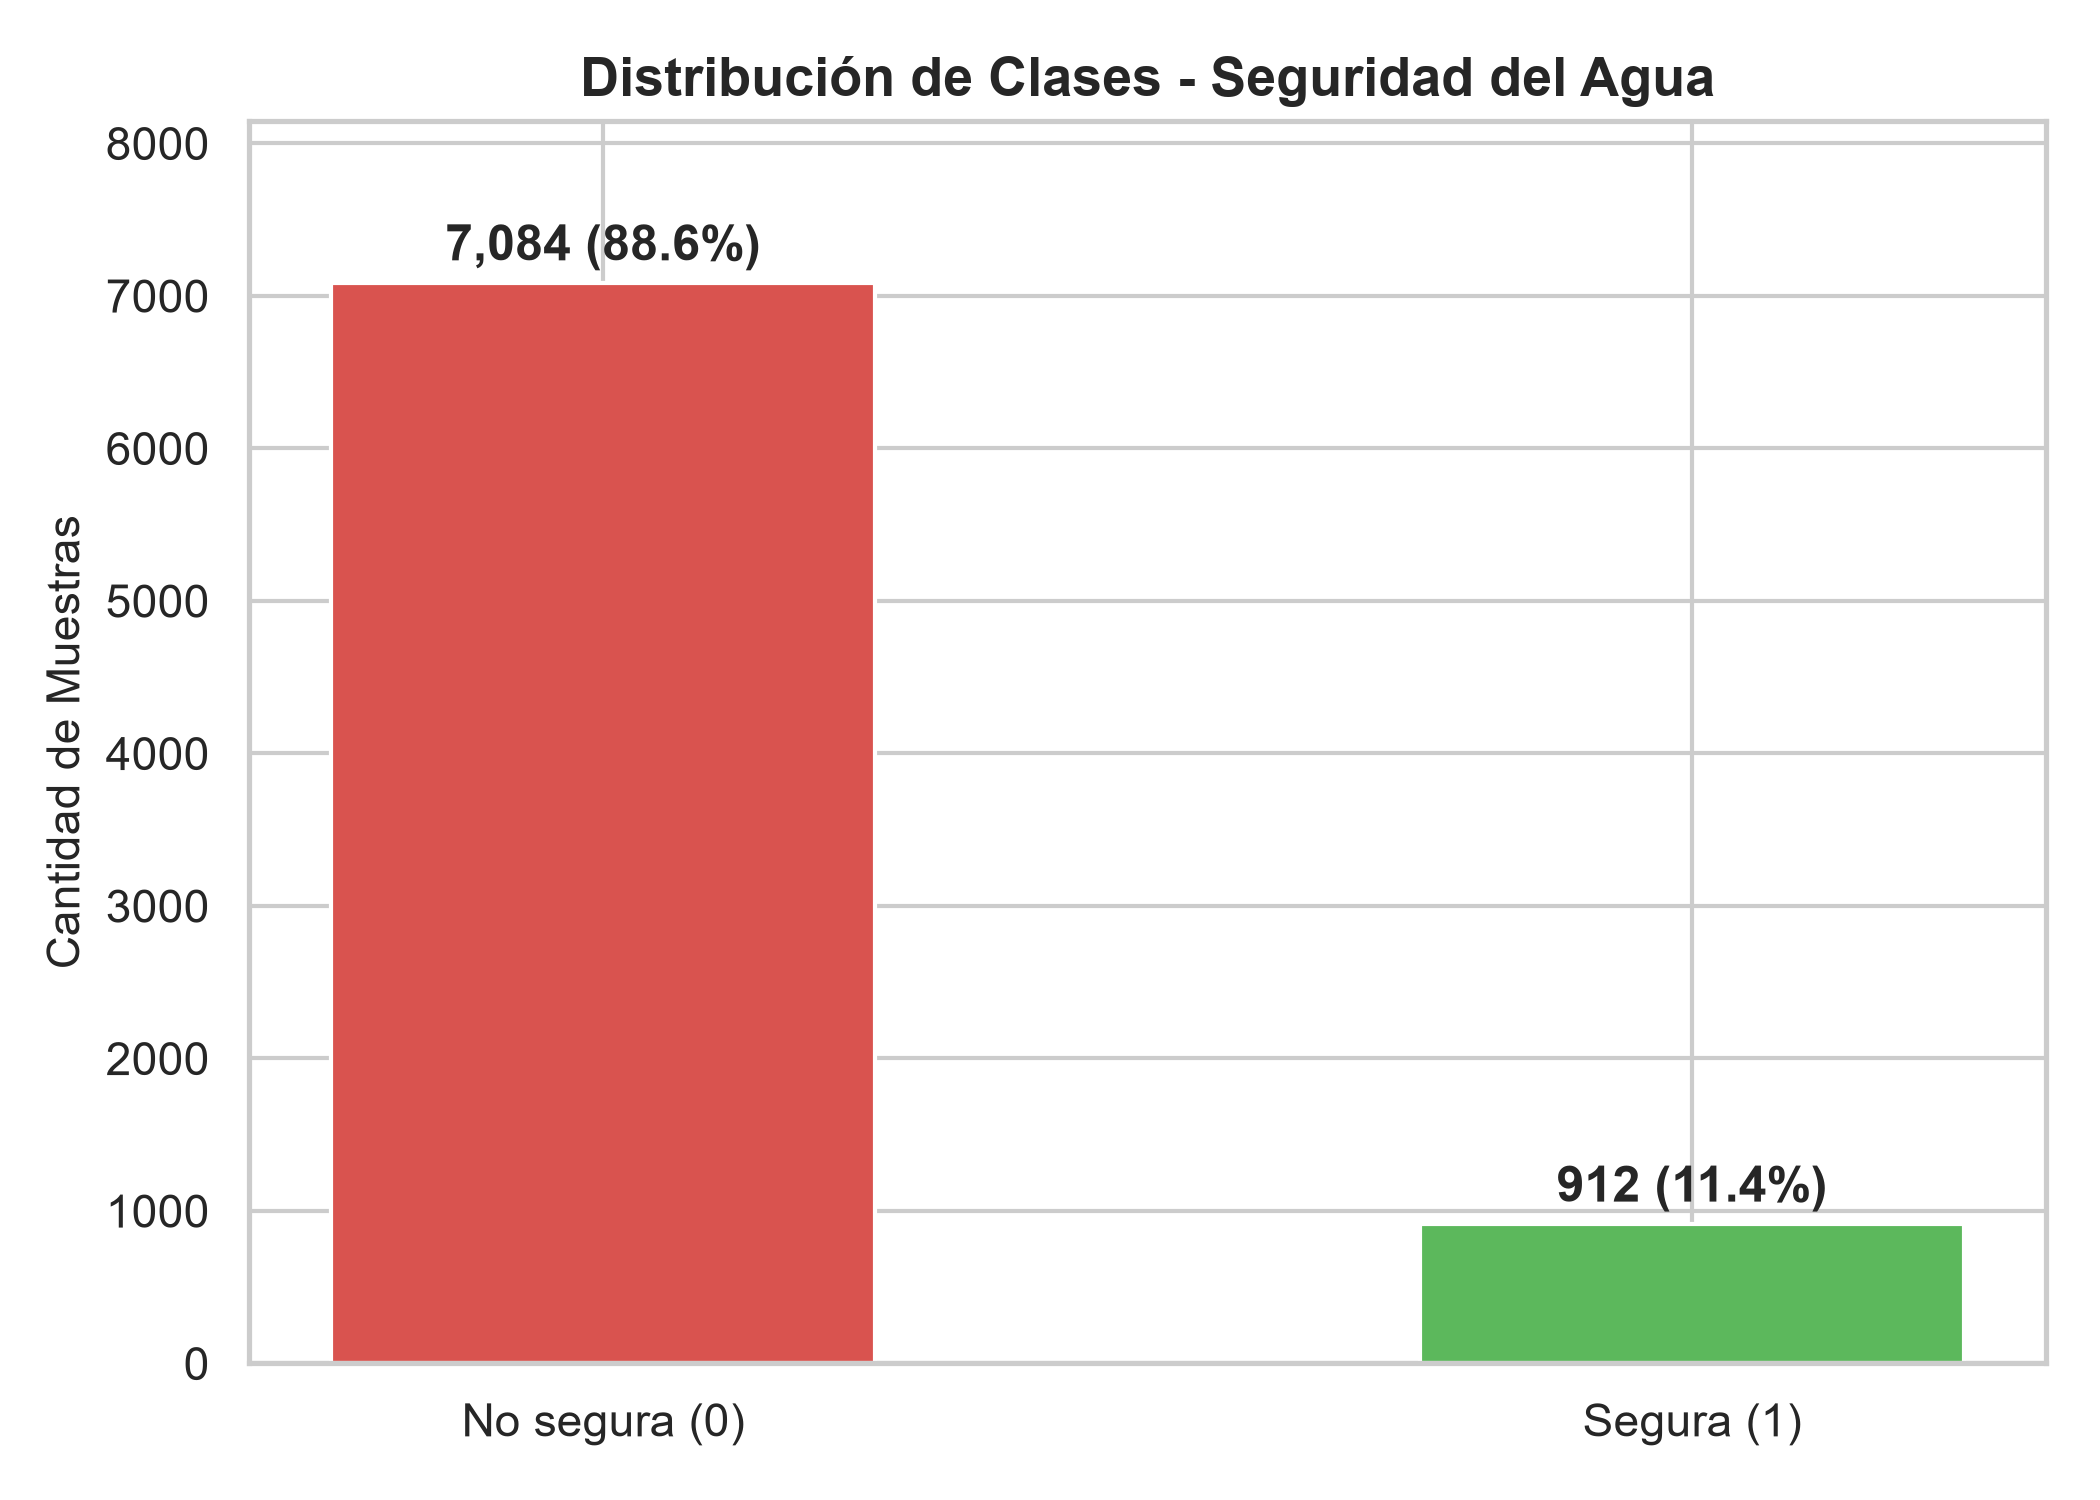
\includegraphics[width=.68\textwidth,height=3.6cm,keepaspectratio]{reports/figures/01_class_distribution.png}\\[0.1cm]
{\small\textbf{Figura 1.} Distribuci\'{o}n de la variable objetivo \textit{is\_safe} en el dataset Water Quality (fuerte desbalance: 88,59\,\% no segura frente a 11,41\,\% segura).}
\end{center}

{\small\renewcommand{\arraystretch}{1.03}\begin{tabularx}{\textwidth}{XXX}
\toprule
Variable & Concepto & Unidad original \\
\midrule
aluminium & Aluminio & Sin verificar \\
ammonia & Amoníaco & Sin verificar \\
arsenic & Arsénico & Sin verificar \\
barium & Bario & Sin verificar \\
cadmium & Cadmio & Sin verificar \\
chloramine & Cloramina & Sin verificar \\
chromium & Cromo & Sin verificar \\
copper & Cobre & Sin verificar \\
flouride & Fluoruro & Sin verificar \\
bacteria & Bacterias & Sin verificar \\
viruses & Virus & Sin verificar \\
lead & Plomo & Sin verificar \\
nitrates & Nitratos & Sin verificar \\
nitrites & Nitritos & Sin verificar \\
mercury & Mercurio & Sin verificar \\
perchlorate & Perclorato & Sin verificar \\
radium & Radio & Sin verificar \\
selenium & Selenio & Sin verificar \\
silver & Plata & Sin verificar \\
uranium & Uranio & Sin verificar \\
\bottomrule\end{tabularx}}

Se conserva flouride, error de escritura original, para compatibilidad con el pipeline. El diccionario identifica conceptos, sin asignar mg/L, CFU/mL, PFU/mL, pCi/L o Bq/L como unidades verificadas. El mínimo de ammonia en train es -0,08: se documenta como anomalía; el prototipo rechaza mediciones negativas sin cambiar el experimento ya cerrado.

\clearpage
\subsection*{Exploraci\'{o}n de correlaciones y metales pesados}
Como parte de la exploraci\'{o}n inicial sobre el conjunto de entrenamiento, se analizaron las correlaciones entre contaminantes y la presencia de metales pesados en las muestras de agua. La Figura 2 expone la matriz de correlaci\'{o}n lineal completa entre las 20 variables, mientras que la Figura 3 detalla la asociaci\'{o}n individual con la etiqueta \textit{is\_safe} y la distribuci\'{o}n por clases para los metales pesados de mayor relevancia toxicol\'{o}gica.

\vspace{0.2cm}
\begin{center}
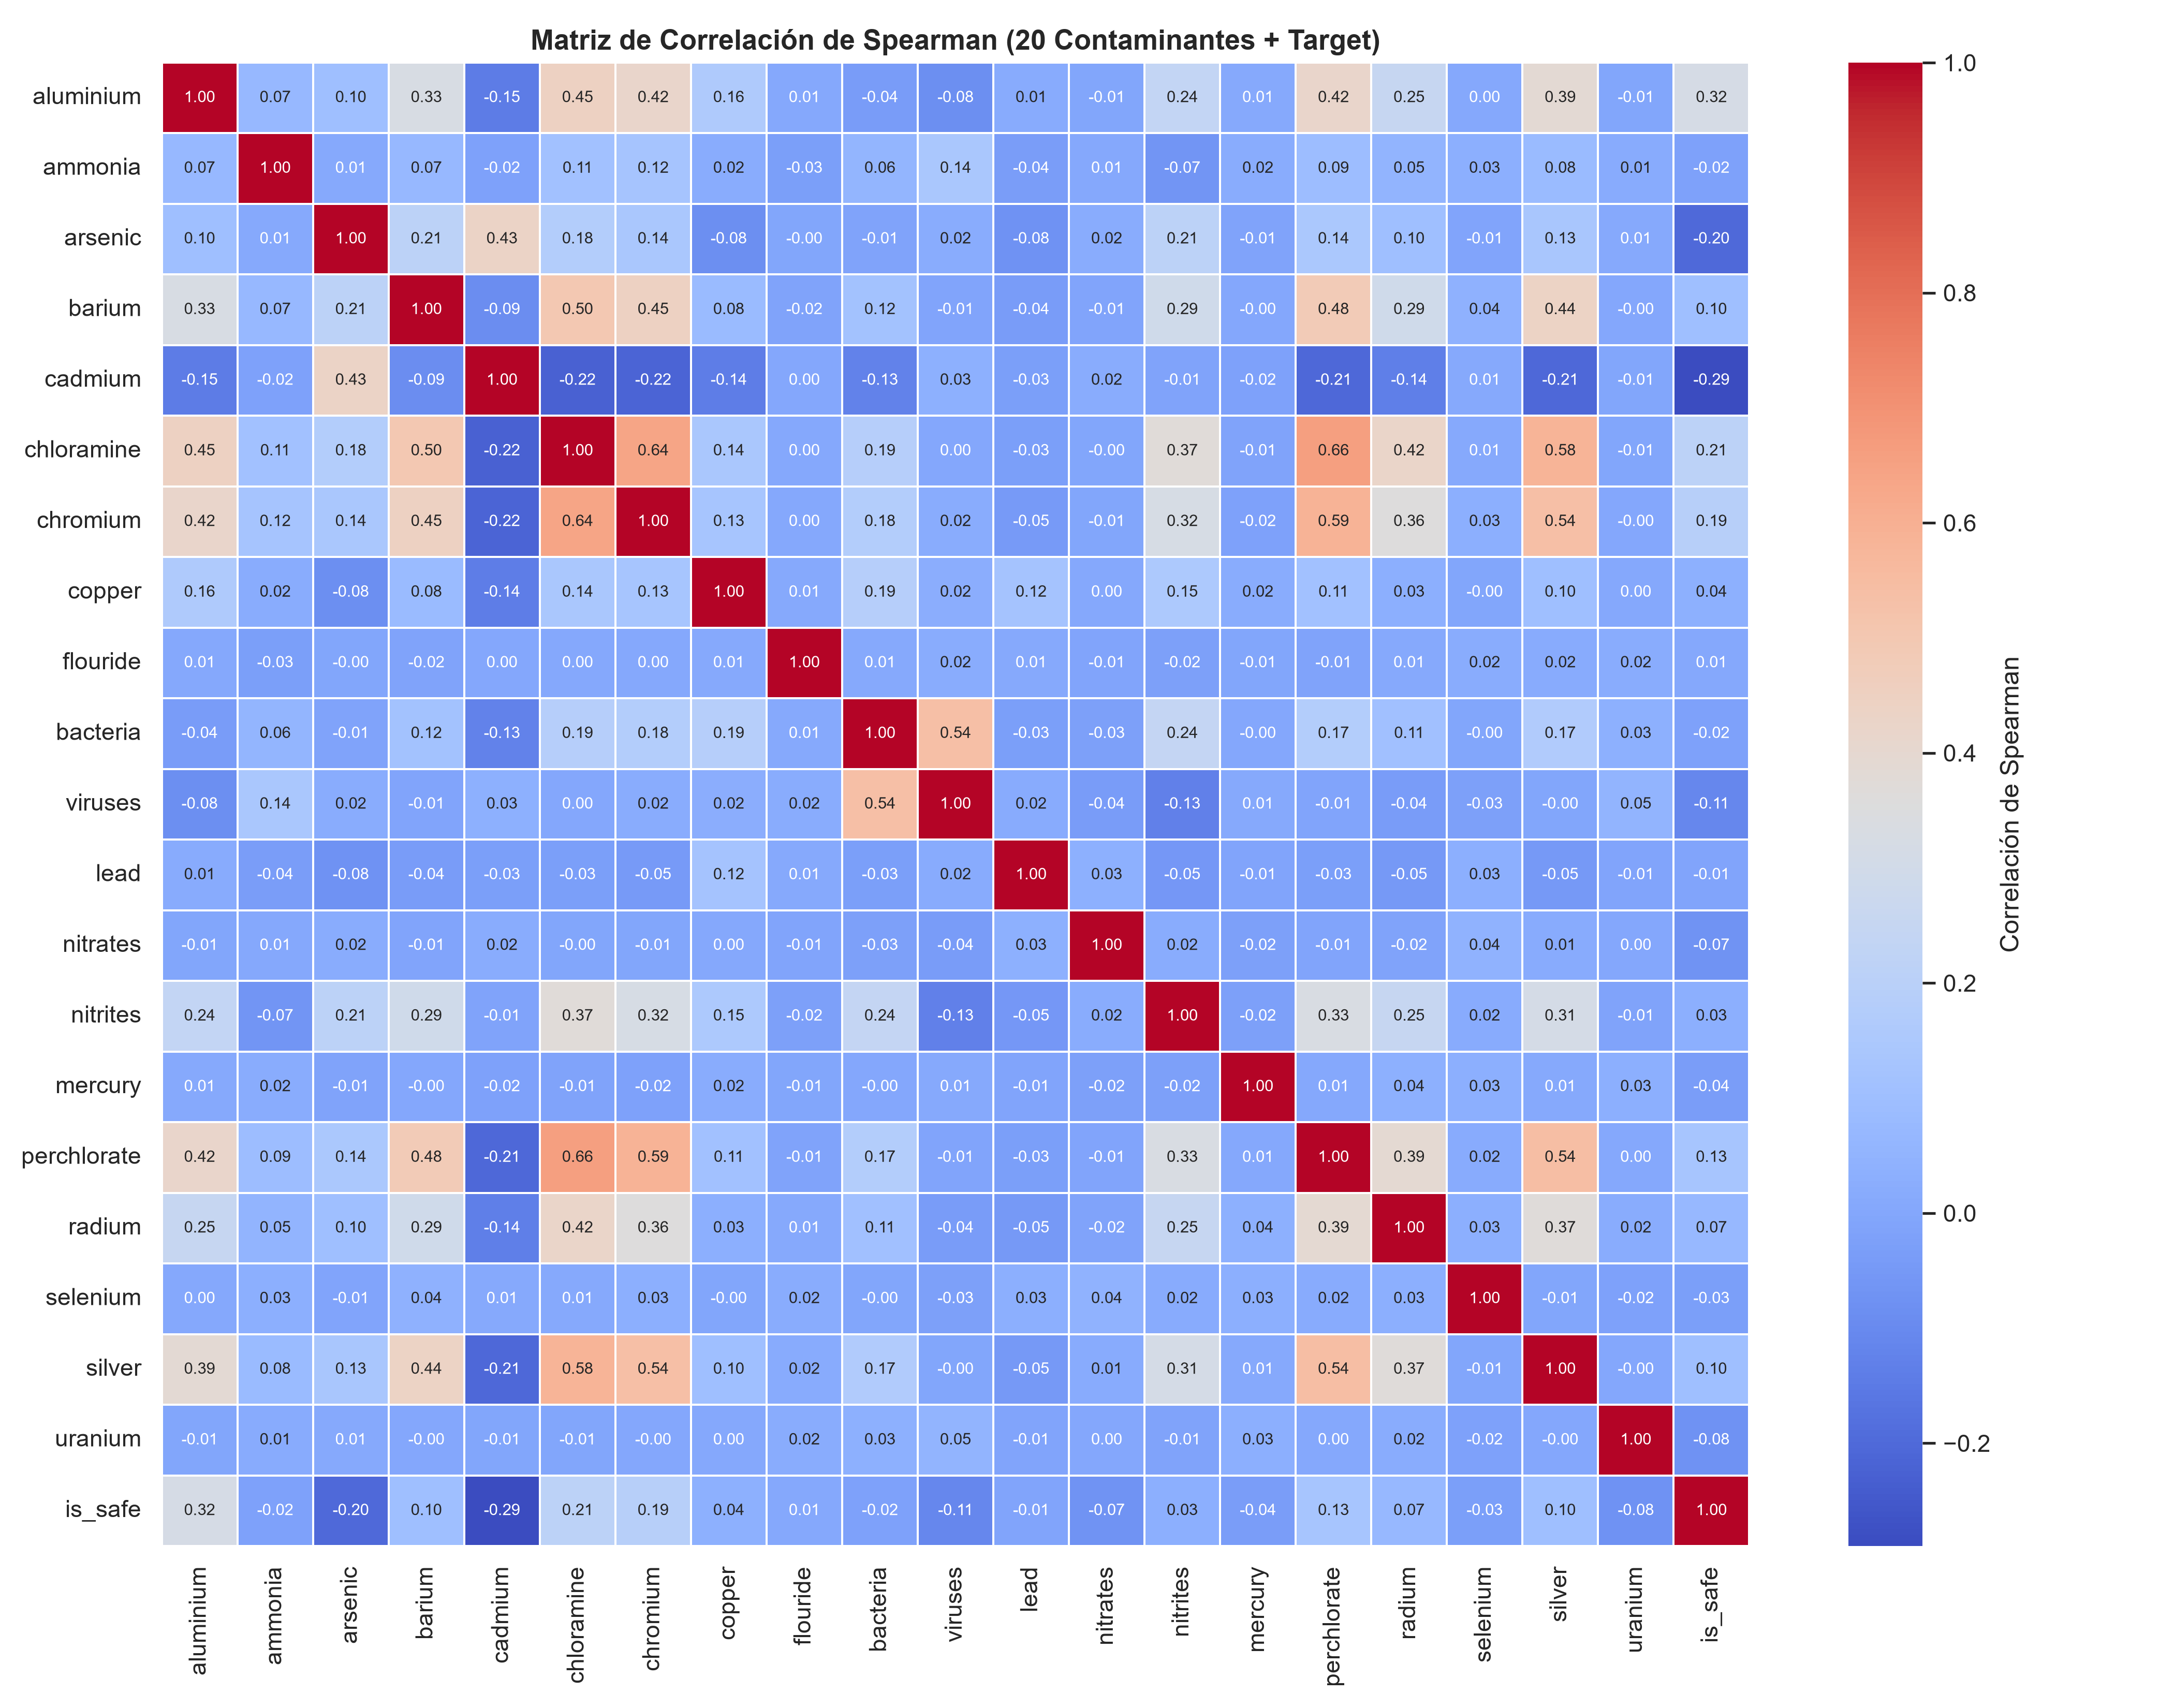
\includegraphics[width=.82\textwidth,height=6.4cm,keepaspectratio]{reports/figures/02_correlation_heatmap.png}\\[0.12cm]
{\small\textbf{Figura 2.} Matriz de correlaci\'{o}n lineal entre las 20 variables fisicoqu\'{i}micas del agua.}
\end{center}

\vspace{0.2cm}
\begin{center}
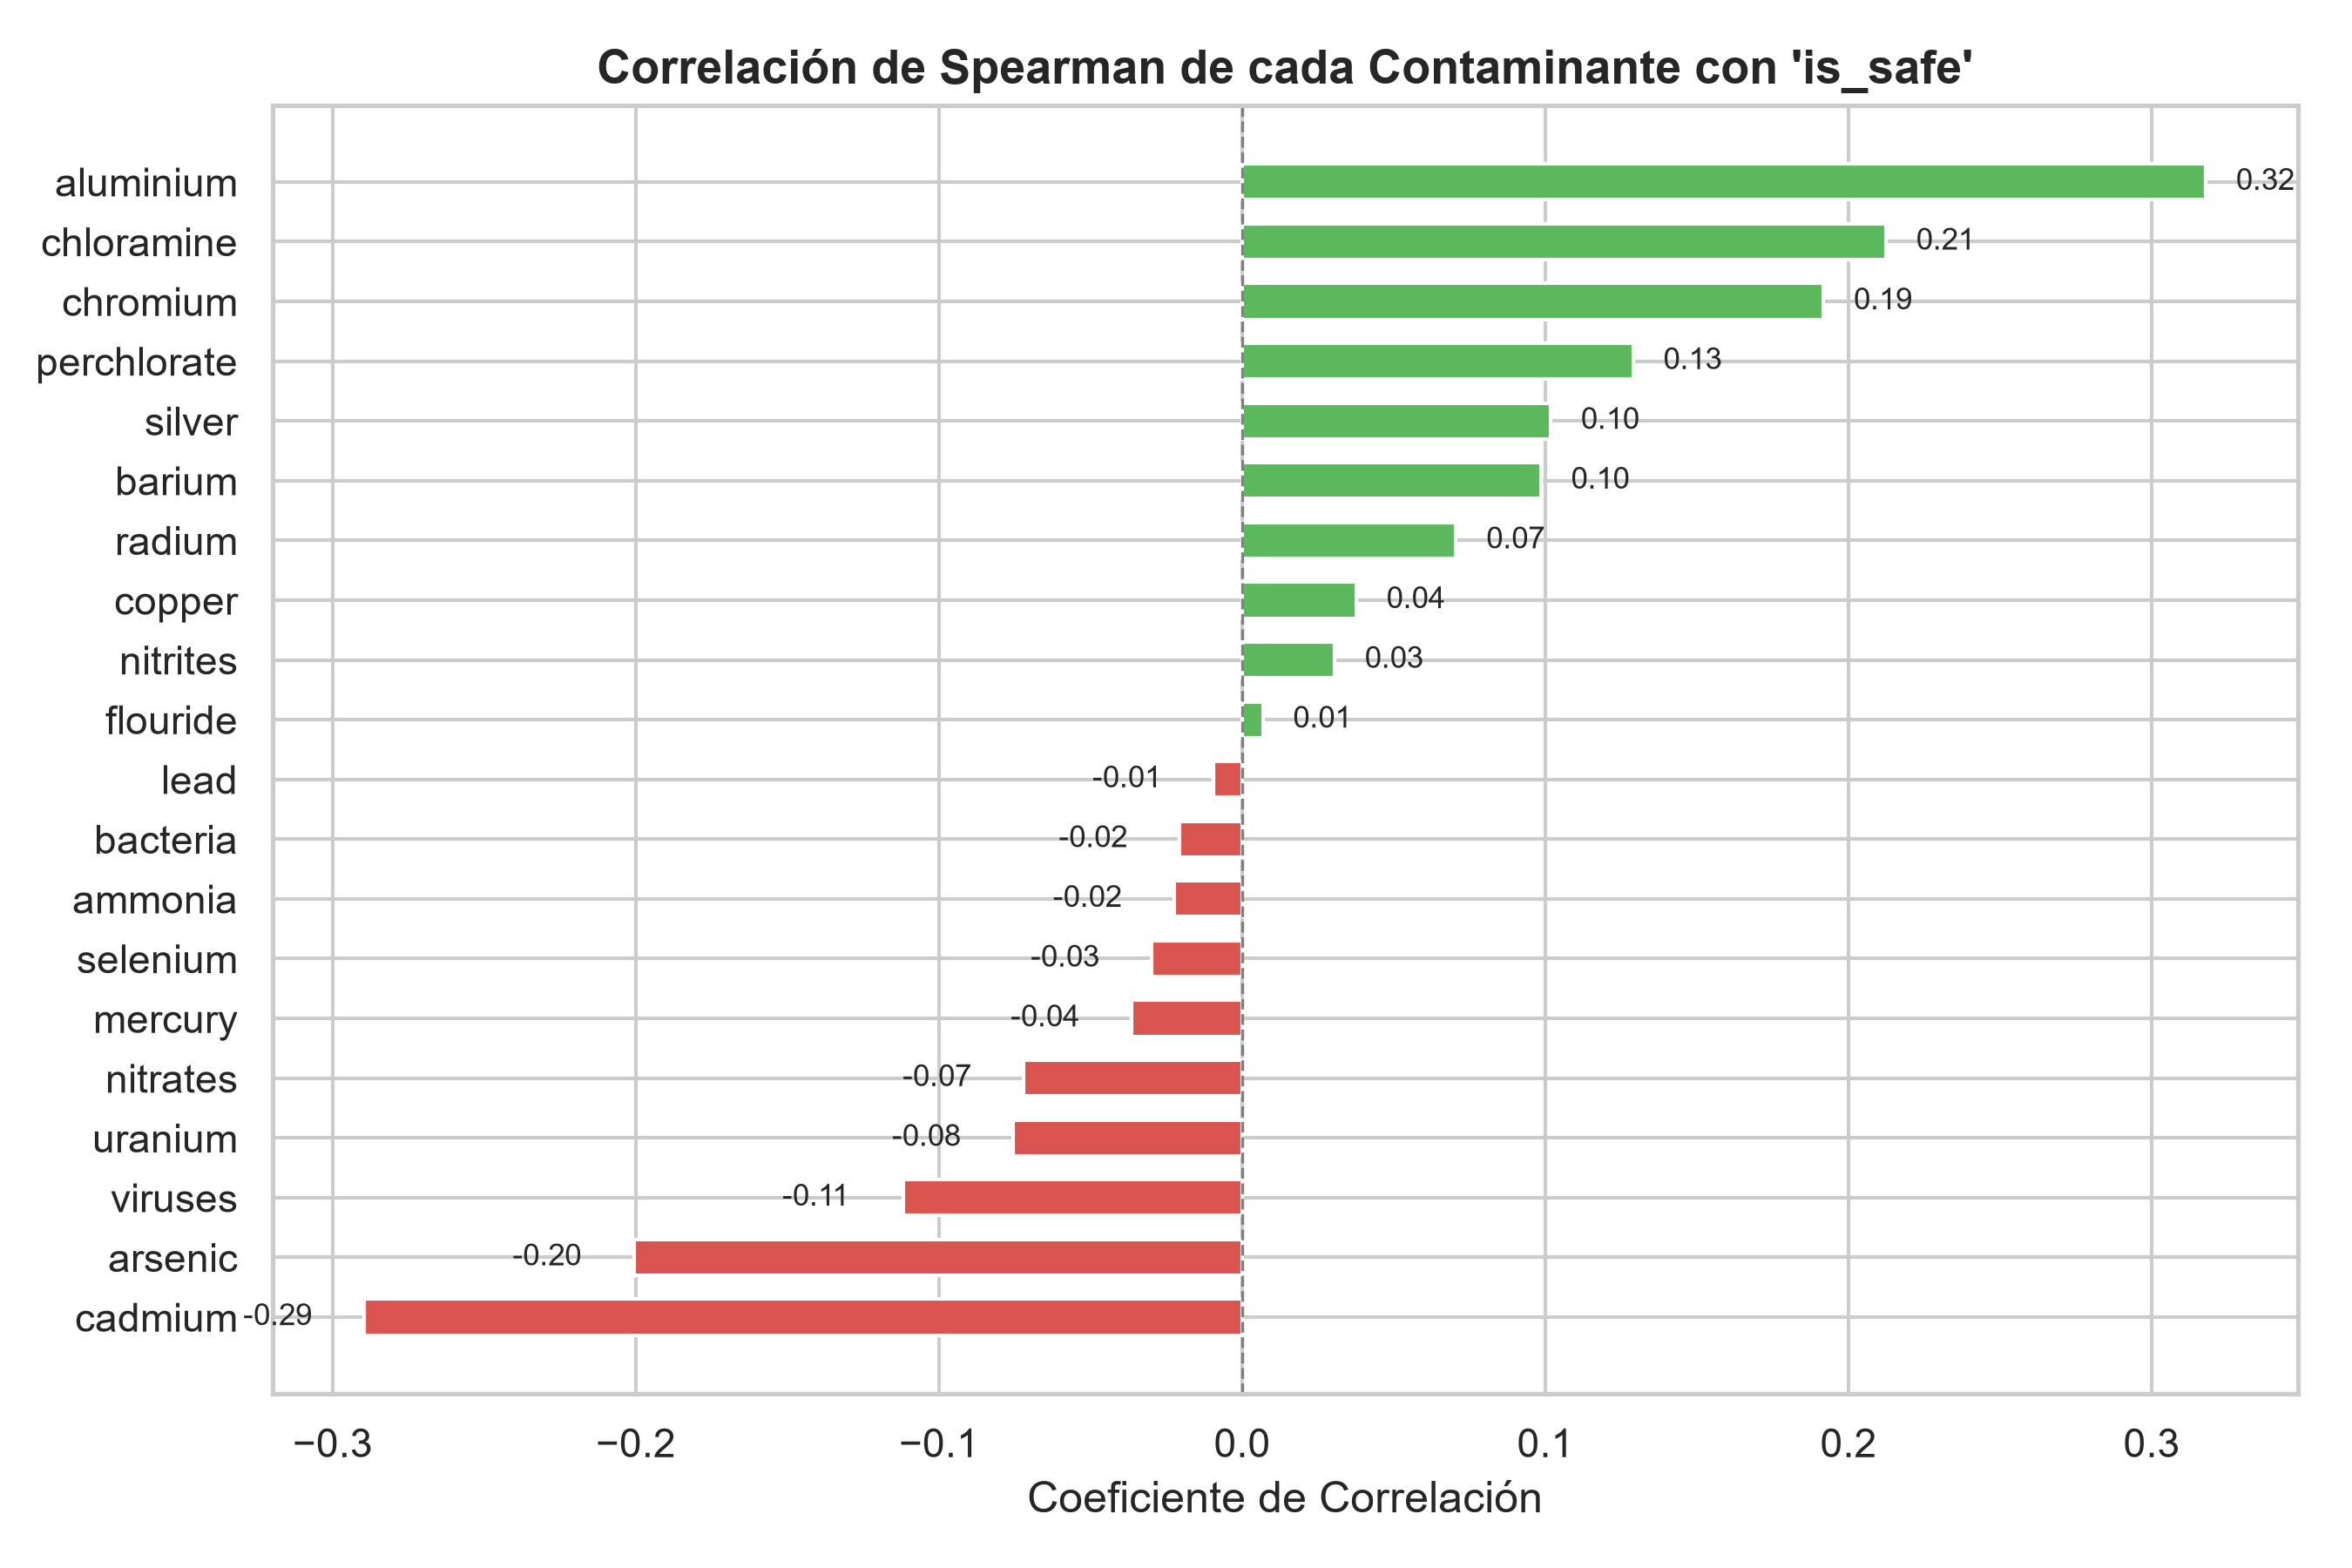
\includegraphics[width=.48\textwidth,height=5.4cm,keepaspectratio]{reports/figures/04_contaminants_correlation_target.png}
\hfill
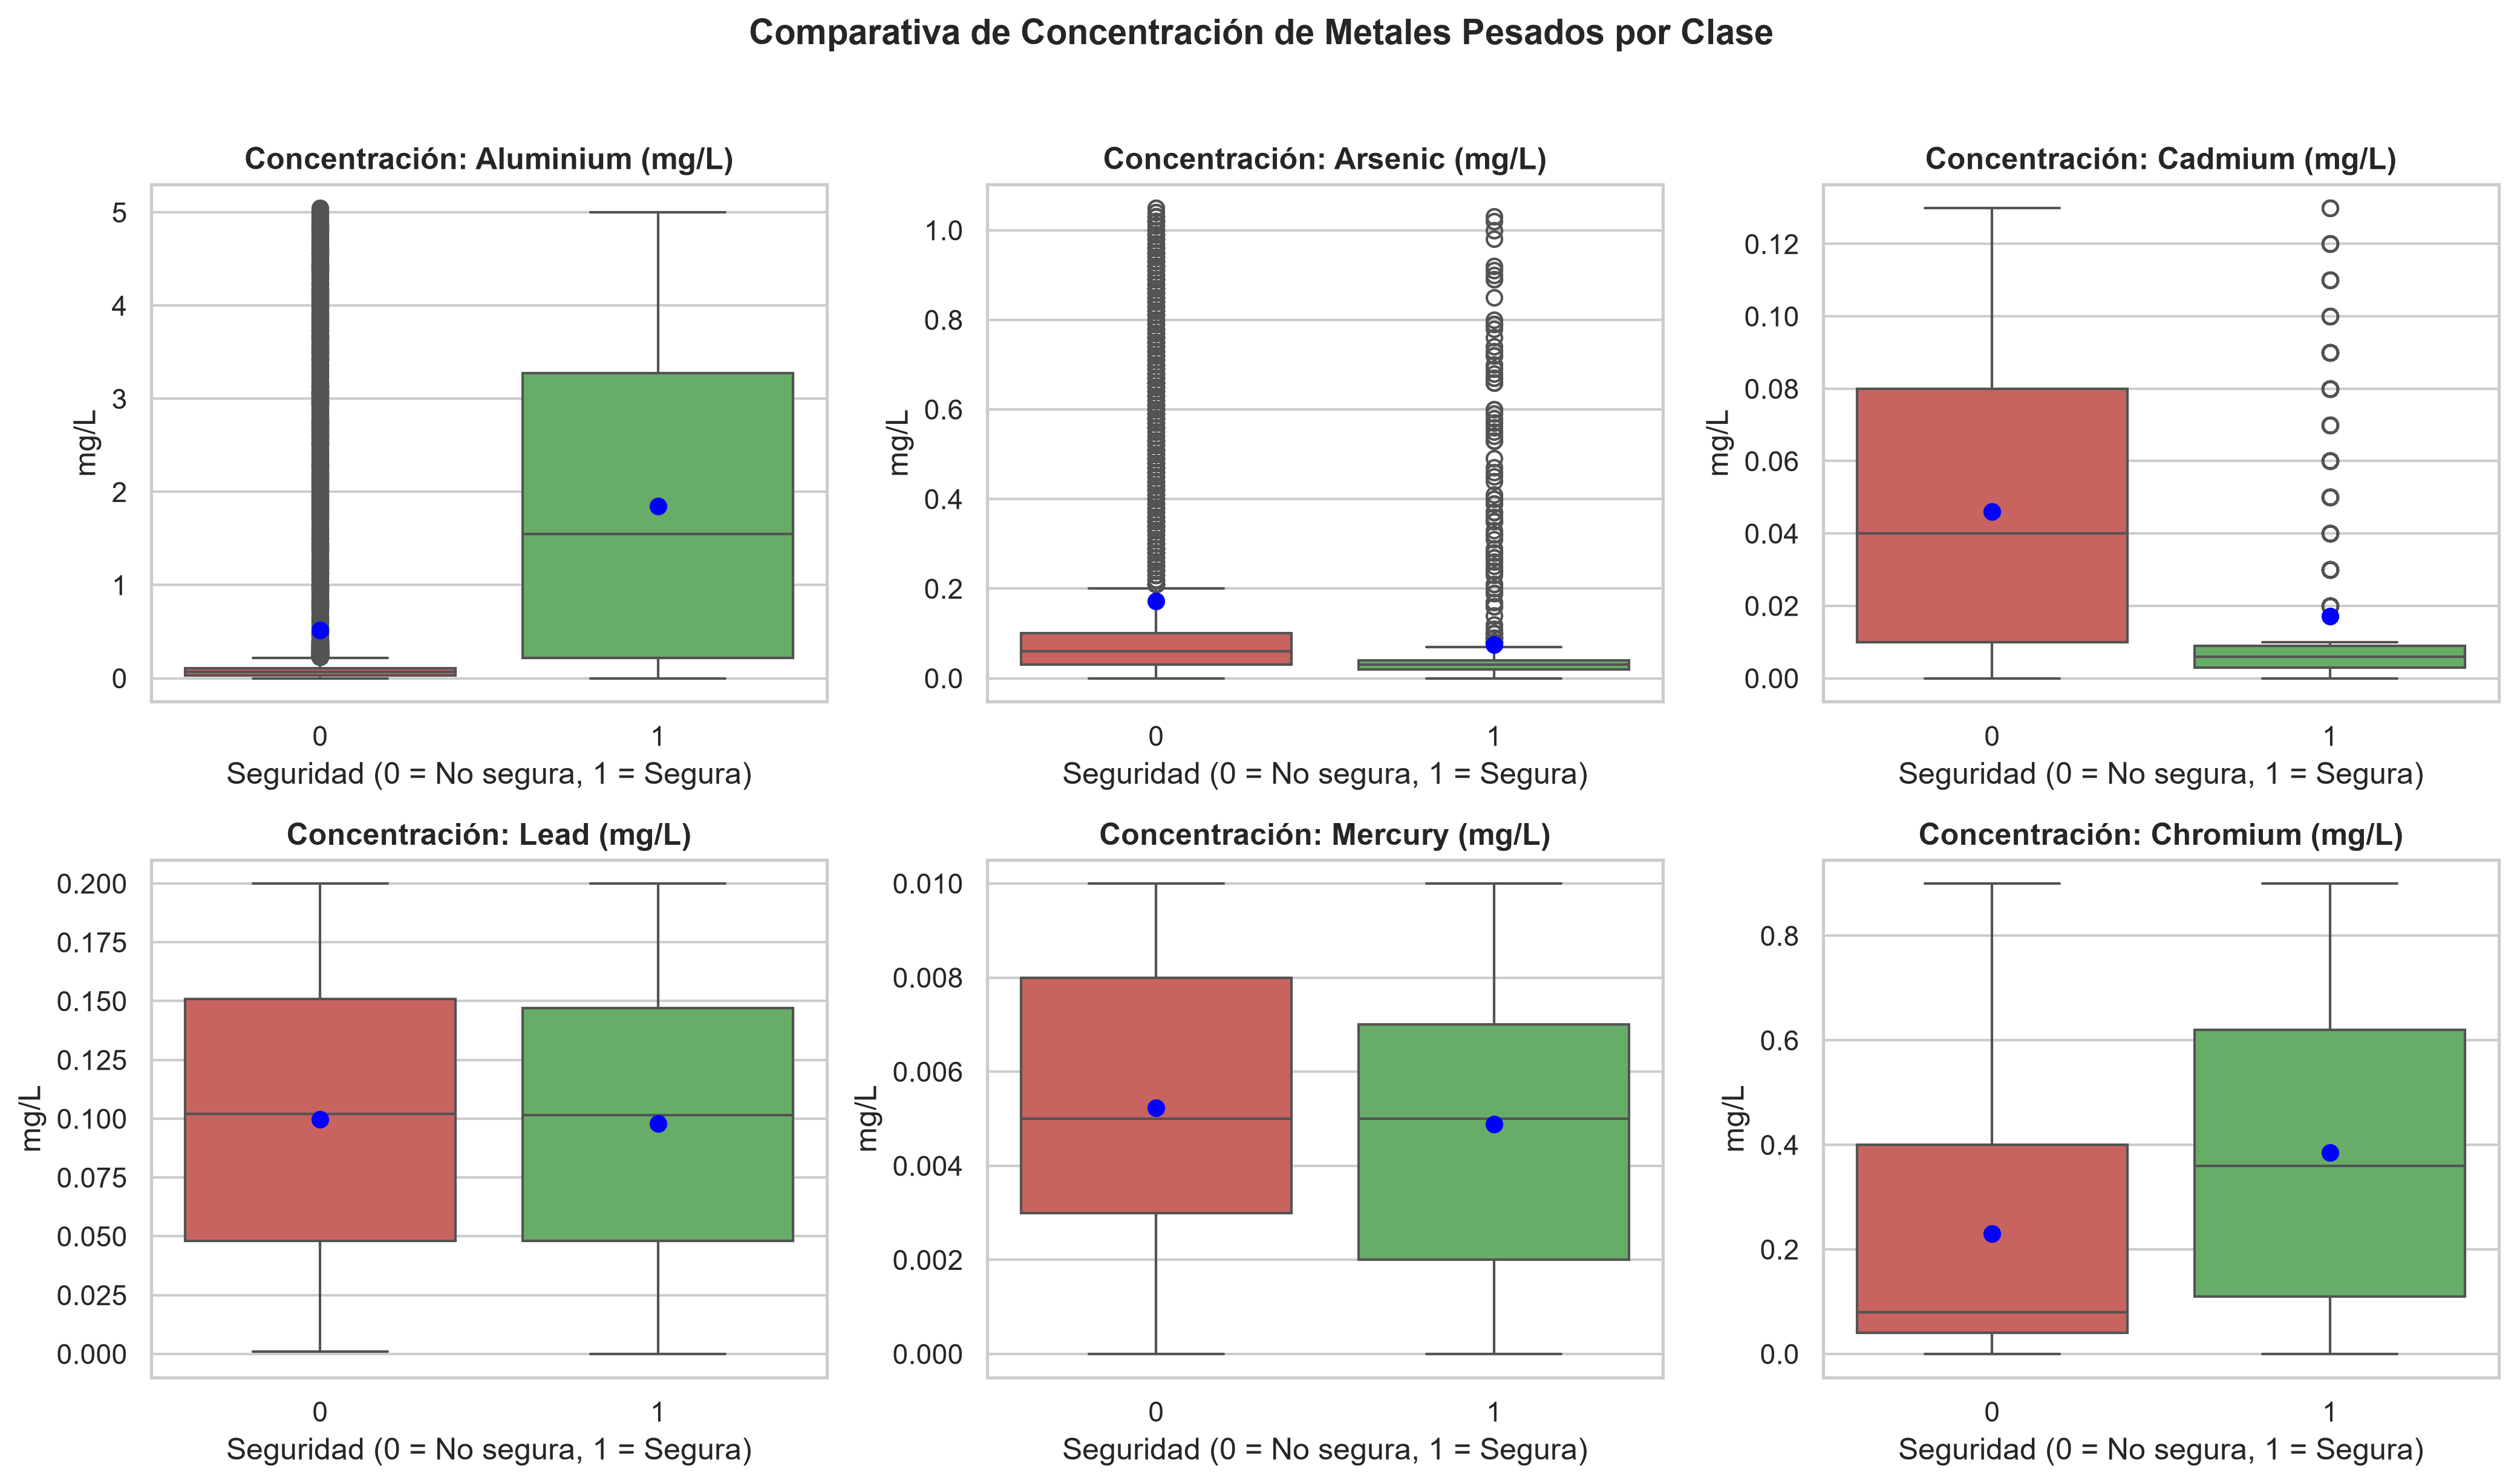
\includegraphics[width=.48\textwidth,height=5.4cm,keepaspectratio]{reports/figures/03_heavy_metals_boxplots.png}\\[0.12cm]
{\small\textbf{Figura 3.} An\'{a}lisis exploratorio de variables: correlaci\'{o}n de contaminantes con \textit{is\_safe} (izquierda) y distribuci\'{o}n en diagramas de caja para metales pesados (derecha).}
\end{center}

\clearpage
\section*{4. Metodología y reproducibilidad}
La limpieza de las tres etiquetas inválidas precedió al split 80/20 estratificado, con semilla 42. En CV se usó StratifiedKFold(n\_splits=5, shuffle=True, random\_state=42). StandardScaler y cada estimador forman un Pipeline: el escalado se ajusta dentro del entrenamiento de cada pliegue. No se usó el preprocesador independiente de fase II para validar los candidatos.

La fase II incluyó exploración descriptiva del conjunto completo antes de la partición. Esto limita cualquier afirmación de sellado absoluto. No se usaron sus estadísticas globales para ajustar escalado ni para modificar hiperparámetros con el test. La documentación de fase IV también registra la lectura del encabezado y una fila de test antes de la evaluación predictiva. Se preserva esa desviación en el informe.

Los candidatos y búsquedas se evaluaron únicamente en train. Se reutilizaron los mismos cinco pliegues para buscar y resumir candidatos optimizados, por lo que sus medias pueden ser optimistas. No se realizó CV anidada. Los espacios de GA y GridSearch son distintos. La comparación describe esas ejecuciones y no identifica el algoritmo globalmente más eficiente.

La configuración RF-GA se fijó antes de calcular las métricas del test. El pipeline final se ajustó a todo train, se persistió y luego se predijo sobre test una sola vez. El archivo phase4\_selection.json registra métricas, clases, hashes y entorno. El guard de phase4\_finalize.py impide repetir la evaluación si ya existe ese reporte. Las correcciones de documentación y UI no vuelven a ejecutar ese script.

{\small\begin{tabularx}{\textwidth}{XX}
\toprule
Elemento & Registro del experimento final \\
\midrule
Semilla & 42 \\
Sistema & Windows-11-10.0.26200-SP0 \\
CPU & Intel64 Family 6 Model 198 Stepping 2, GenuineIntel \\
CPU lógicas & 24 \\
Python / NumPy & 3.13.13 / 2.5.1 \\
pandas / scikit-learn & 3.0.5 / 1.9.0 \\
joblib / matplotlib & 1.5.3 / 3.11.2 \\
\bottomrule\end{tabularx}}

El dataset no incluye aquí marcas temporales o identificadores de fuente que permitan comprobar independencia por entidad o validación cronológica. La partición aleatoria no prueba generalización a nuevas plantas, regiones o períodos. Antes de una aplicación ambiental real se necesita nueva evidencia externa con unidades y procedencia verificadas.

\clearpage
\section*{5. Comparación en validación cruzada}
Fuente: reports/phase3\_results.json. Los valores son media $\pm$ desviación estándar de cinco pliegues sobre train. Recall y precision corresponden a la clase 1 (segura según etiquetas). El ROC-AUC usa el score de clase 1. La desviación entre pliegues no constituye un intervalo de confianza.

{\small\begin{tabularx}{\textwidth}{XXXXX}
\toprule
Modelo & Macro-F1 & ROC-AUC & Recall(1) & Precision(1) \\
\midrule
Dummy & 0.4697 $\pm$ 0.0000 & 0.5000 $\pm$ 0.0000 & 0.0000 $\pm$ 0.0000 & 0.0000 $\pm$ 0.0000 \\
KNN & 0.6975 $\pm$ 0.0214 & 0.8656 $\pm$ 0.0096 & 0.3644 $\pm$ 0.0550 & 0.6016 $\pm$ 0.0496 \\
SVM RBF & 0.8207 $\pm$ 0.0159 & 0.9557 $\pm$ 0.0072 & 0.7808 $\pm$ 0.0237 & 0.6149 $\pm$ 0.0302 \\
RF base & 0.8863 $\pm$ 0.0135 & 0.9839 $\pm$ 0.0033 & 0.8795 $\pm$ 0.0215 & 0.7359 $\pm$ 0.0274 \\
MLP & 0.8509 $\pm$ 0.0251 & 0.9643 $\pm$ 0.0132 & 0.6507 $\pm$ 0.0616 & 0.8425 $\pm$ 0.0517 \\
RF-GA & 0.8967 $\pm$ 0.0132 & 0.9868 $\pm$ 0.0033 & 0.8603 $\pm$ 0.0311 & 0.7802 $\pm$ 0.0214 \\
RF-Grid & 0.8979 $\pm$ 0.0119 & 0.9870 $\pm$ 0.0028 & 0.8849 $\pm$ 0.0218 & 0.7657 $\pm$ 0.0226 \\
\bottomrule\end{tabularx}}

Dummy predice siempre la clase mayoritaria y obtiene Macro-F1 0,4697, pese a su accuracy 0,8859. RF base y ambas variantes optimizadas presentan las mayores medias de Macro-F1 en esta comparación. Las cifras no prueban causalidad ambiental ni superioridad estadística entre configuraciones cercanas.

{\small\begin{tabularx}{\textwidth}{XXX}
\toprule
Modelo & Ajuste (s/pliegue) & Inferencia (ms/lote) \\
\midrule
Dummy & 0.0007 & 0.099 \\
KNN & 0.0032 & 353.868 \\
SVM RBF & 0.1531 & 72.099 \\
RF base & 0.1276 & 28.949 \\
MLP & 0.4849 & 1.615 \\
RF-GA & 0.2296 & 27.694 \\
RF-Grid & 0.2378 & 27.688 \\
\bottomrule\end{tabularx}}

Los tiempos de ajuste son segundos por pliegue. La inferencia es predict sobre el lote de validación (aproximadamente 1.279 registros), expresada en milisegundos y sin incluir predict\_proba. El registro original no conserva desviaciones de tiempos. Se evita presentar estos valores como latencia por muestra o mezclarlos con la duración total de búsqueda.

Configuraciones iniciales: KNN k=7 y weights=distance; SVM RBF C=5, gamma=scale y class\_weight=balanced; RF 100 árboles, max\_depth=12 y class\_weight=balanced; MLP (64,32), ReLU, Adam, max\_iter=250 y early\_stopping=True. El CSV complementario conserva todas las métricas guardadas, incluida accuracy como indicador secundario.

\clearpage
\subsection*{Visualizaci\'{o}n comparativa de modelos}
La Figura 4 sintetiza visualmente la comparaci\'{o}n entre los modelos base y las variantes optimizadas evaluadas en validaci\'{o}n cruzada. Se observa con claridad la brecha sustancial que separa al baseline Dummy de los modelos no lineales, as\'{i} como la proximidad competitiva alcanzada entre el bosque base, la configuraci\'{o}n con Algoritmo Gen\'{e}tico (RF-GA) y la optimizaci\'{o}n exhaustiva (RF-Grid).

\vspace{0.4cm}
\begin{center}
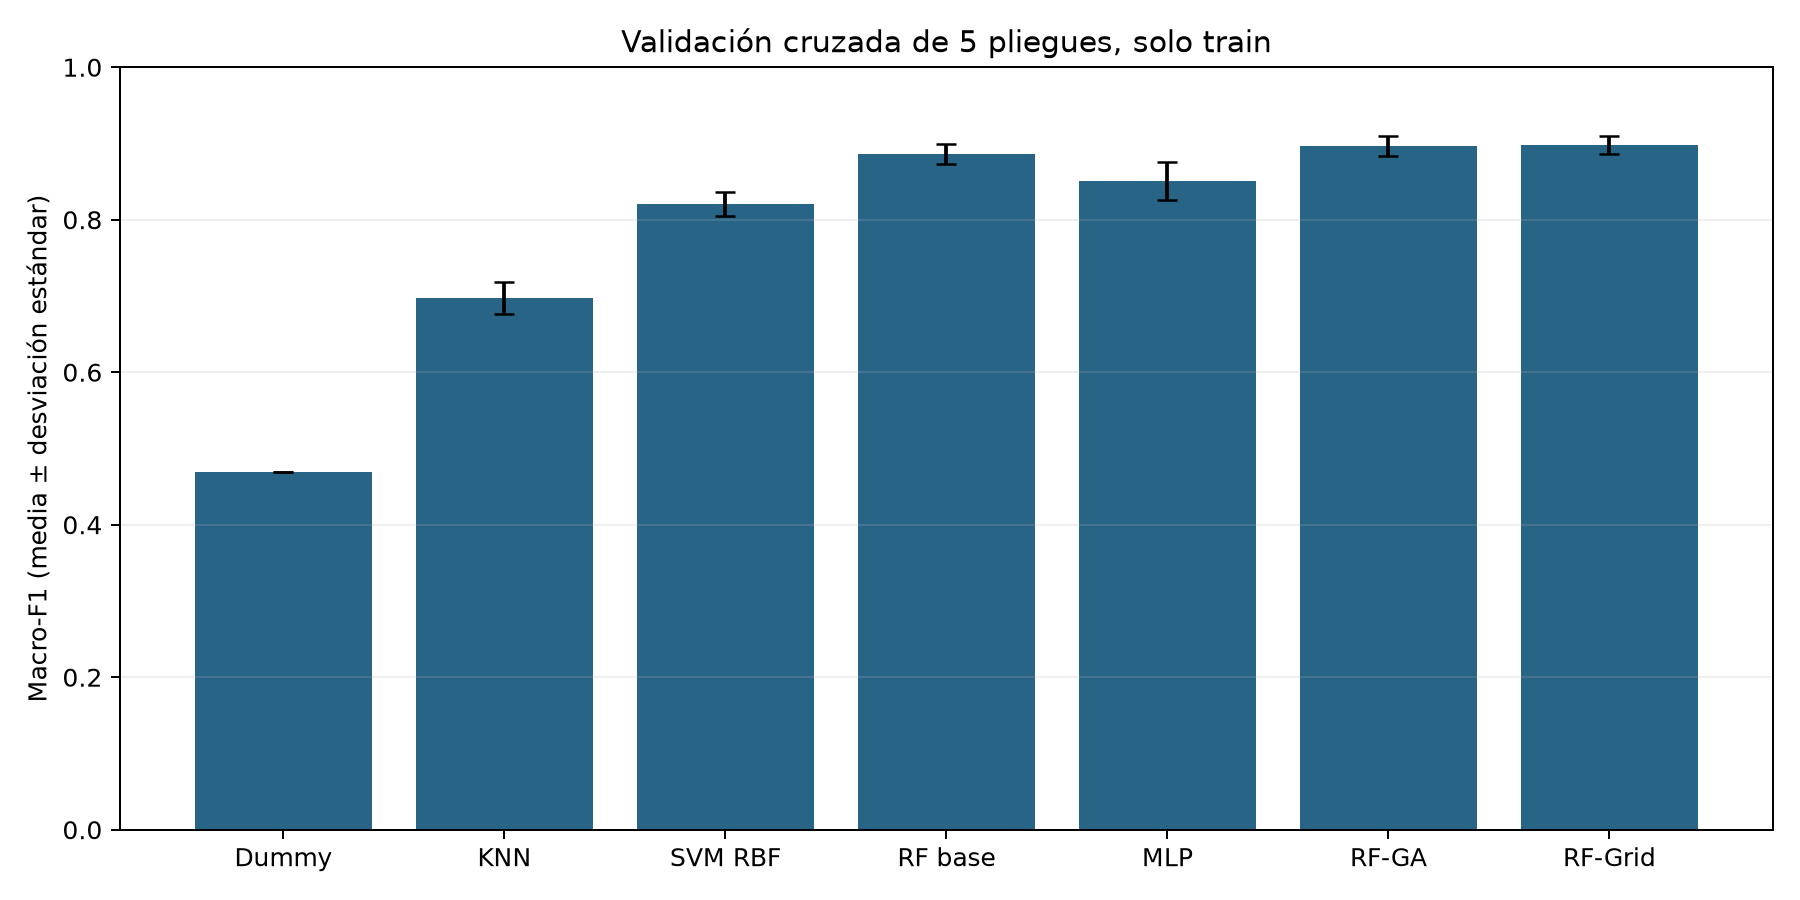
\includegraphics[width=.88\textwidth,height=6.2cm,keepaspectratio]{reports/figures/05_model_comparison_metrics.png}\\[0.15cm]
{\small\textbf{Figura 4.} Comparaci\'{o}n de m\'{e}tricas clave (Macro-F1, ROC-AUC, Recall y Precision) en validaci\'{o}n cruzada de 5 pliegues sobre el conjunto de entrenamiento.}
\end{center}

\clearpage
\section*{6. Optimización y elección del modelo}
El GA empleó 10 individuos durante 5 generaciones, selección por torneo binario, cruce uniforme, mutación de probabilidad 0,25 y 2 élites. La aptitud fue la media de Macro-F1 de CV. La mejor aptitud generacional pasó de 0,8940 a 0,8967. La media poblacional no fue monótona.

\begin{center}
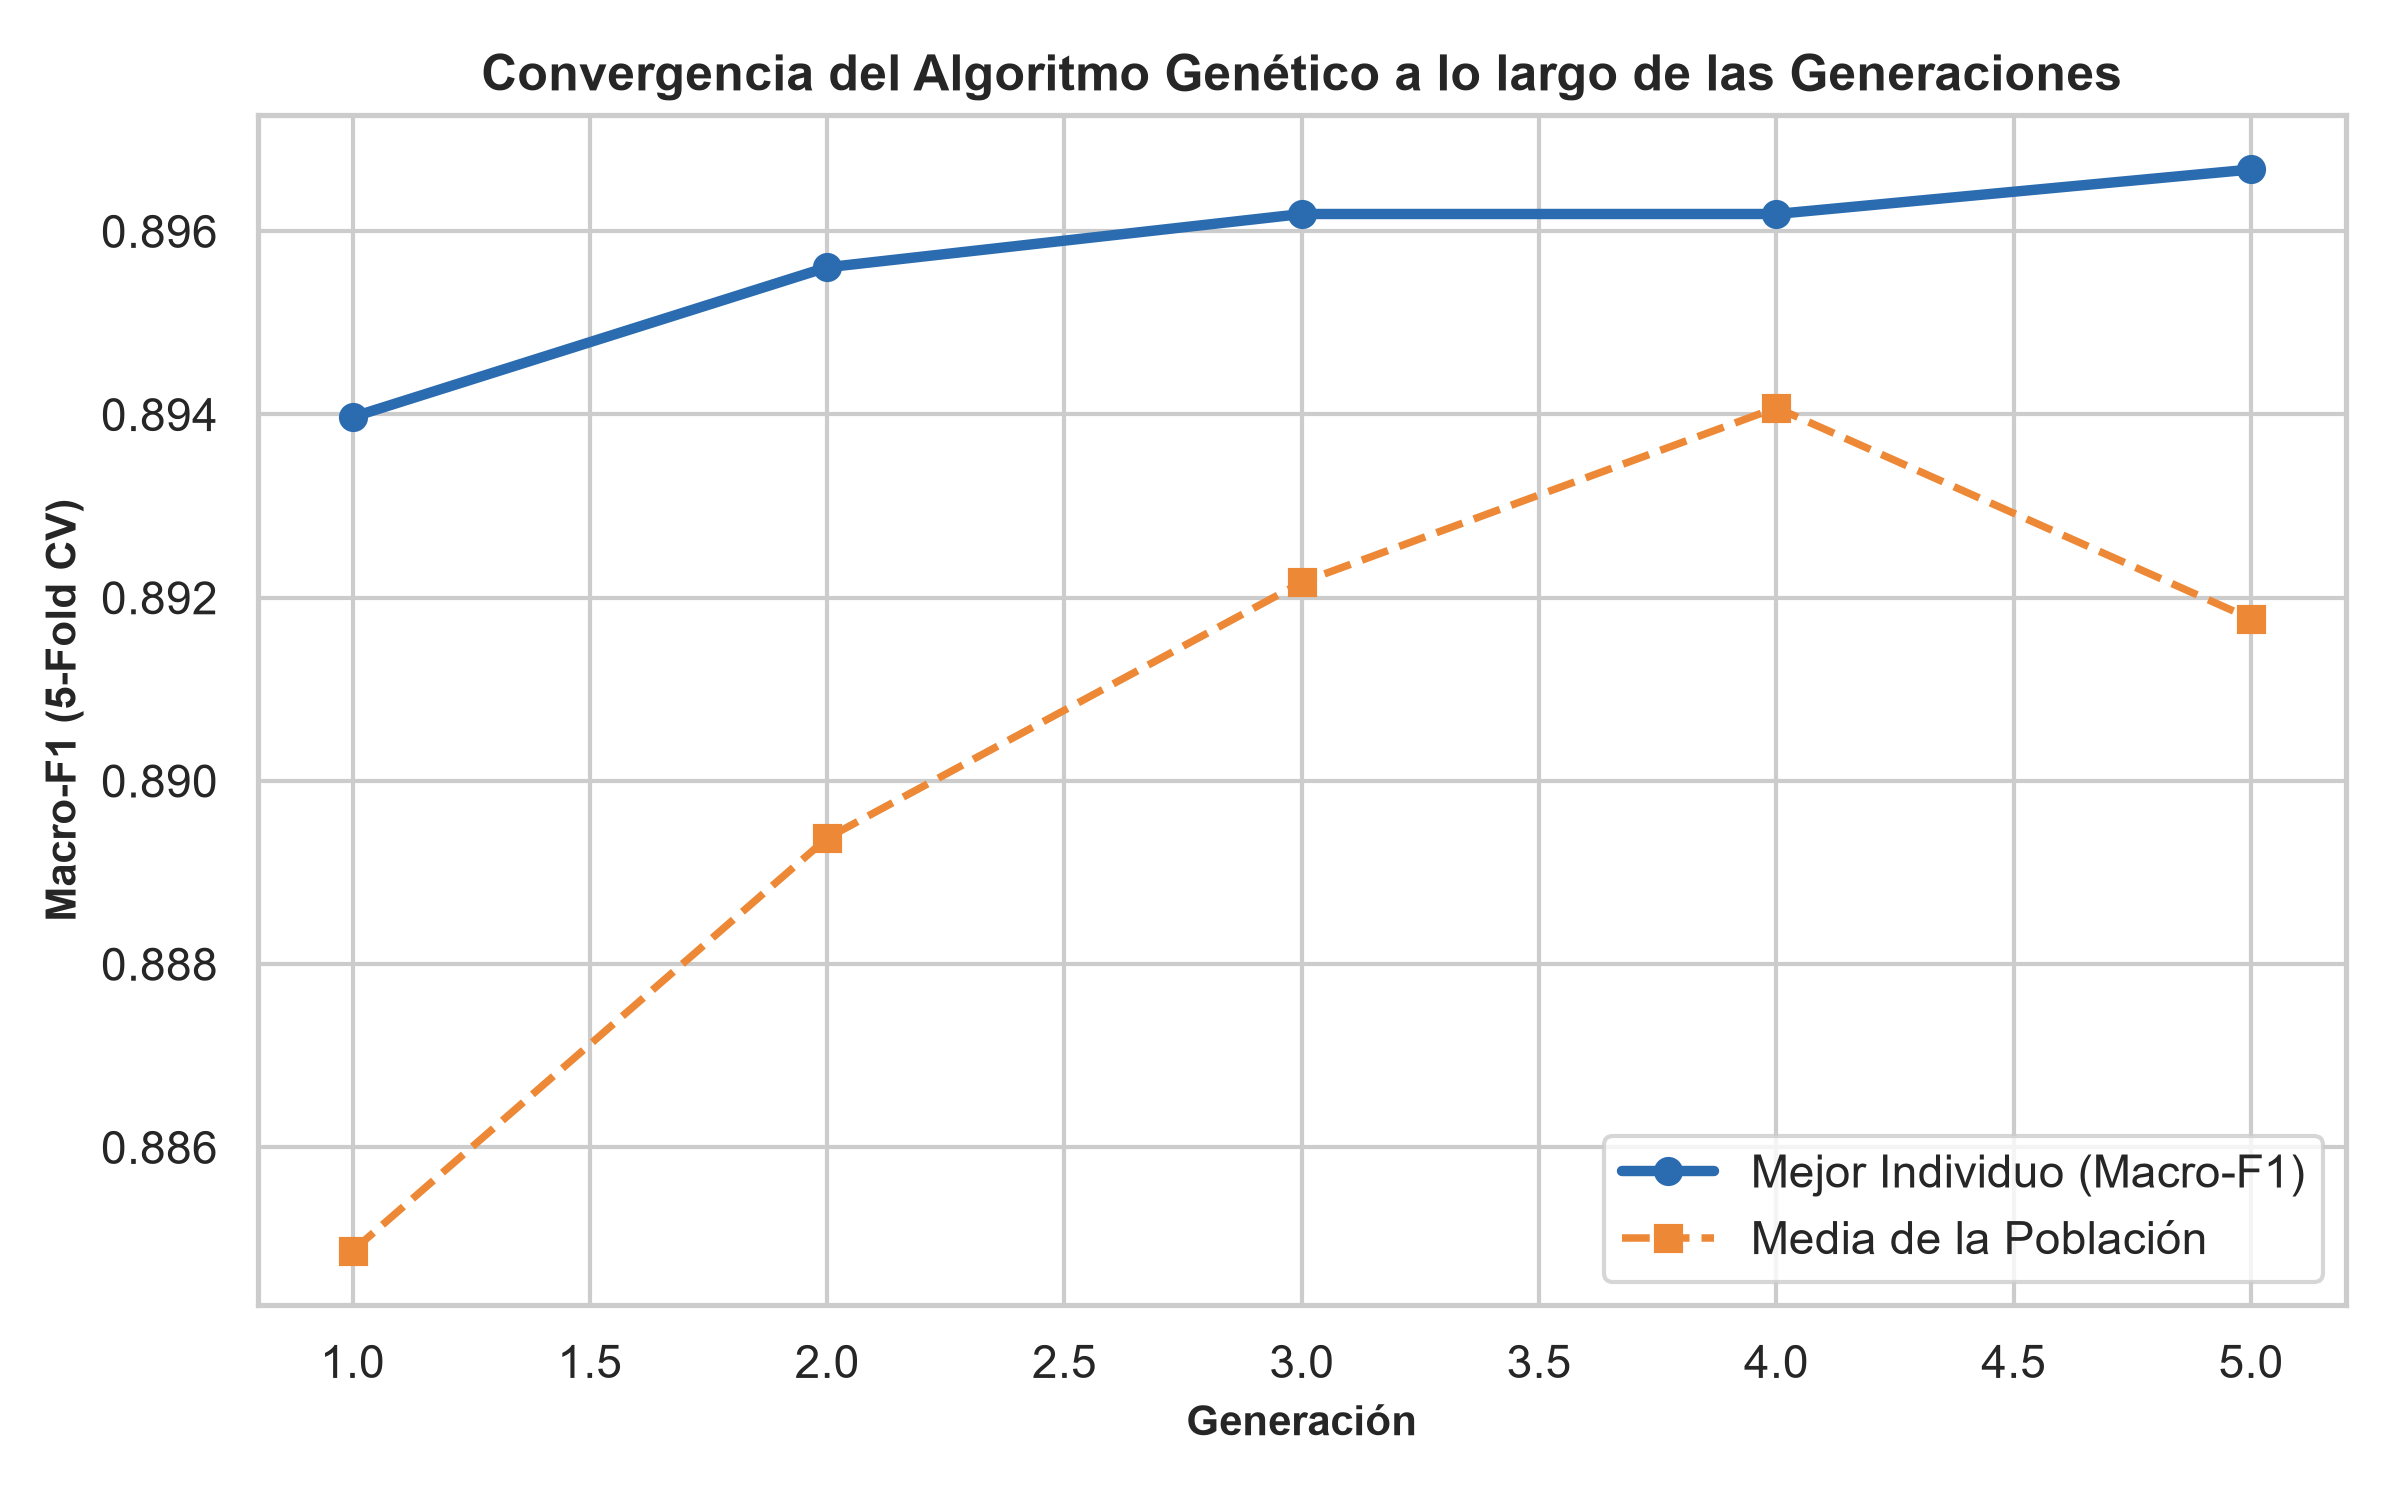
\includegraphics[width=.72\textwidth,height=3.8cm,keepaspectratio]{reports/figures/06_ga_convergence.png}\\[0.1cm]
{\small\textbf{Figura 5.} Curva de convergencia generacional del Algoritmo Gen\'{e}tico (aptitud promedio y m\'{a}xima por generaci\'{o}n en CV).}
\end{center}

\vspace{-0.2cm}
{\small\begin{tabularx}{\textwidth}{XXX}
\toprule
Configuración & RF-GA seleccionado & RF-Grid \\
\midrule
Árboles & 200 & 200 \\
max\_depth & 20 & 14 \\
min\_samples\_split & 4 & 2 \\
min\_samples\_leaf & 1 & 1 \\
criterion / pesos & entropy / balanced & entropy / balanced \\
Macro-F1 CV & 0,8967 $\pm$ 0,0132 & 0,8979 $\pm$ 0,0119 \\
Búsqueda total (s) & 58.46 & 7.79 \\
\bottomrule\end{tabularx}}

GridSearch evaluó 16 combinaciones con árboles [100,200], profundidades [8,14], mínimos para dividir [2,6] y criterios gini/entropy. Su mayor media supera al GA por 0,0012 y su búsqueda registrada fue más rápida. La dispersión no permite declarar equivalencia estadística ni ausencia de diferencia.

Se conservó RF-GA para materializar el eje de optimización metaheurística con desempeño cercano. Esta elección académica está registrada antes del test y no se presenta como victoria numérica del GA. Los otros modelos tuvieron menor media de Macro-F1. La revisión actual mantiene la configuración y el pipeline congelados.

\begin{center}
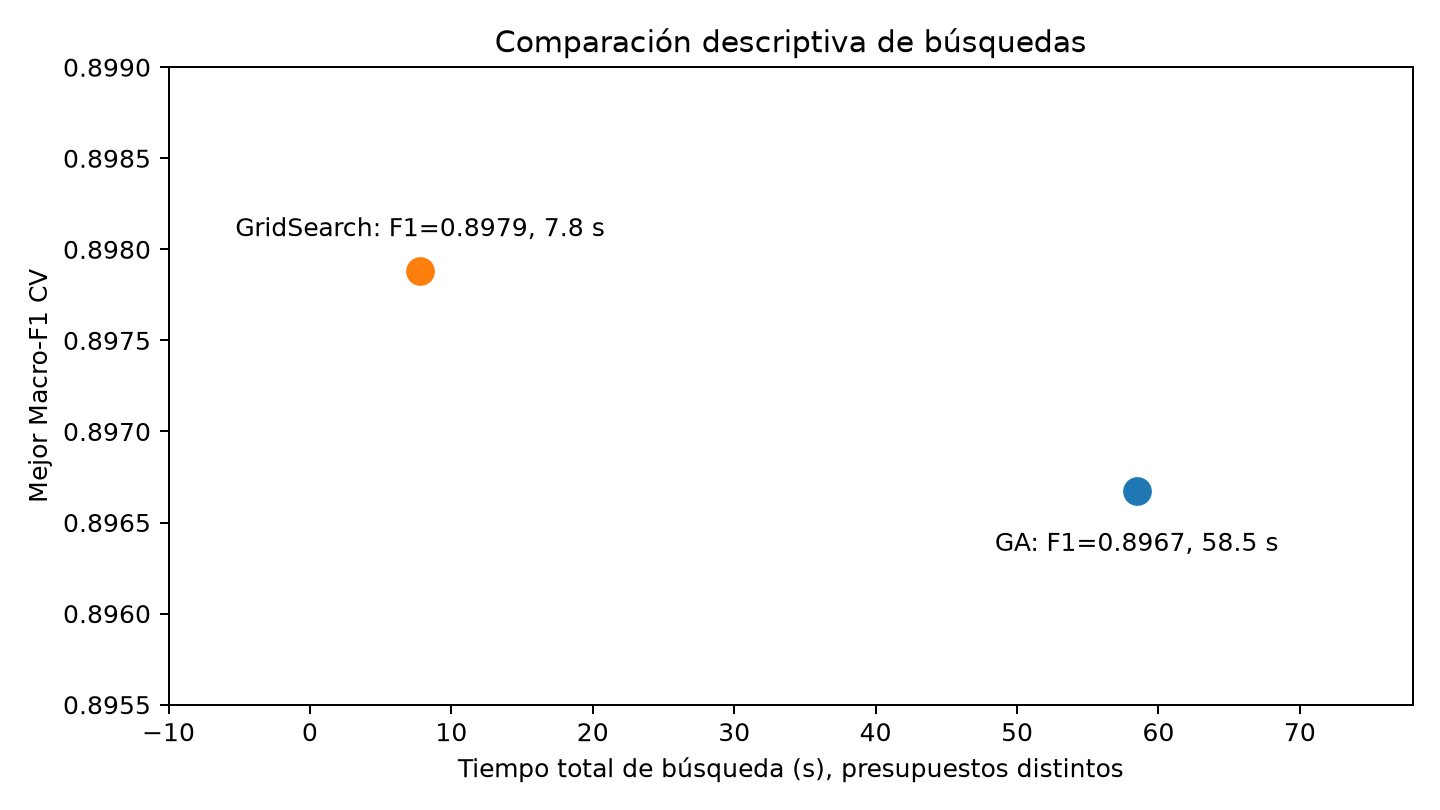
\includegraphics[width=.72\textwidth,height=3.8cm,keepaspectratio]{reports/figures/07_ga_vs_grid_tradeoff.png}\\[0.1cm]
{\small\textbf{Figura 6.} Comparaci\'{o}n de trade-off de optimizaci\'{o}n entre Algoritmo Gen\'{e}tico y GridSearch (Macro-F1 alcanzado vs tiempo total de b\'{u}squeda).}
\end{center}

\clearpage
\section*{7. Evaluación final y análisis de errores}
Fuente: reports/phase4\_selection.json. Una evaluación predictiva sobre 1.600 registros tras fijar el candidato. Filas: clase real. Columnas: predicción. La clase positiva convencional es la 1, segura según el dataset.

{\small\begin{tabularx}{\textwidth}{XXX}
\toprule
Real / Predicha & No segura (0) & Segura (1) \\
\midrule
No segura (0) & 1.386 & 32 \\
Segura (1) & 30 & 152 \\
\bottomrule\end{tabularx}}

{\small\begin{tabularx}{\textwidth}{XX}
\toprule
Métrica de test & Resultado \\
\midrule
Macro-F1 & 0.9044 \\
ROC-AUC, clase 1 & 0.9829 \\
Recall clase 0, no segura & 0.9774 \\
Precision clase 0, no segura & 0.9788 \\
Recall clase 1, segura & 0.8352 \\
Precision clase 1, segura & 0.8261 \\
Accuracy complementaria & 0.9613 \\
\bottomrule\end{tabularx}}

El error de mayor preocupación para una interpretación sanitaria es clasificar 32 muestras realmente no seguras como seguras: 32/1.418 = 2,26 \% de la clase 0 del test. Con clase positiva 1, esos casos son falsos positivos. No deben llamarse falsos negativos sin redefinir explícitamente la clase positiva.

Las otras 30 muestras tenían etiqueta segura y se predijeron no seguras. También son errores y pueden generar costos de verificación o descarte. No se afirma que este comportamiento sea siempre deseable ni que la etiqueta segura sea evidencia de potabilidad real.

El Macro-F1 final (0,9044) es cercano al de CV de RF-GA (0,8967 $\pm$ 0,0132), pero la comparación no demuestra estabilidad en otras poblaciones. Las métricas resumen una partición y no proporcionan garantía de riesgo individual. ROC-AUC mide ordenación de scores, no calibración de probabilidades.

\vspace{0.2cm}
\begin{center}
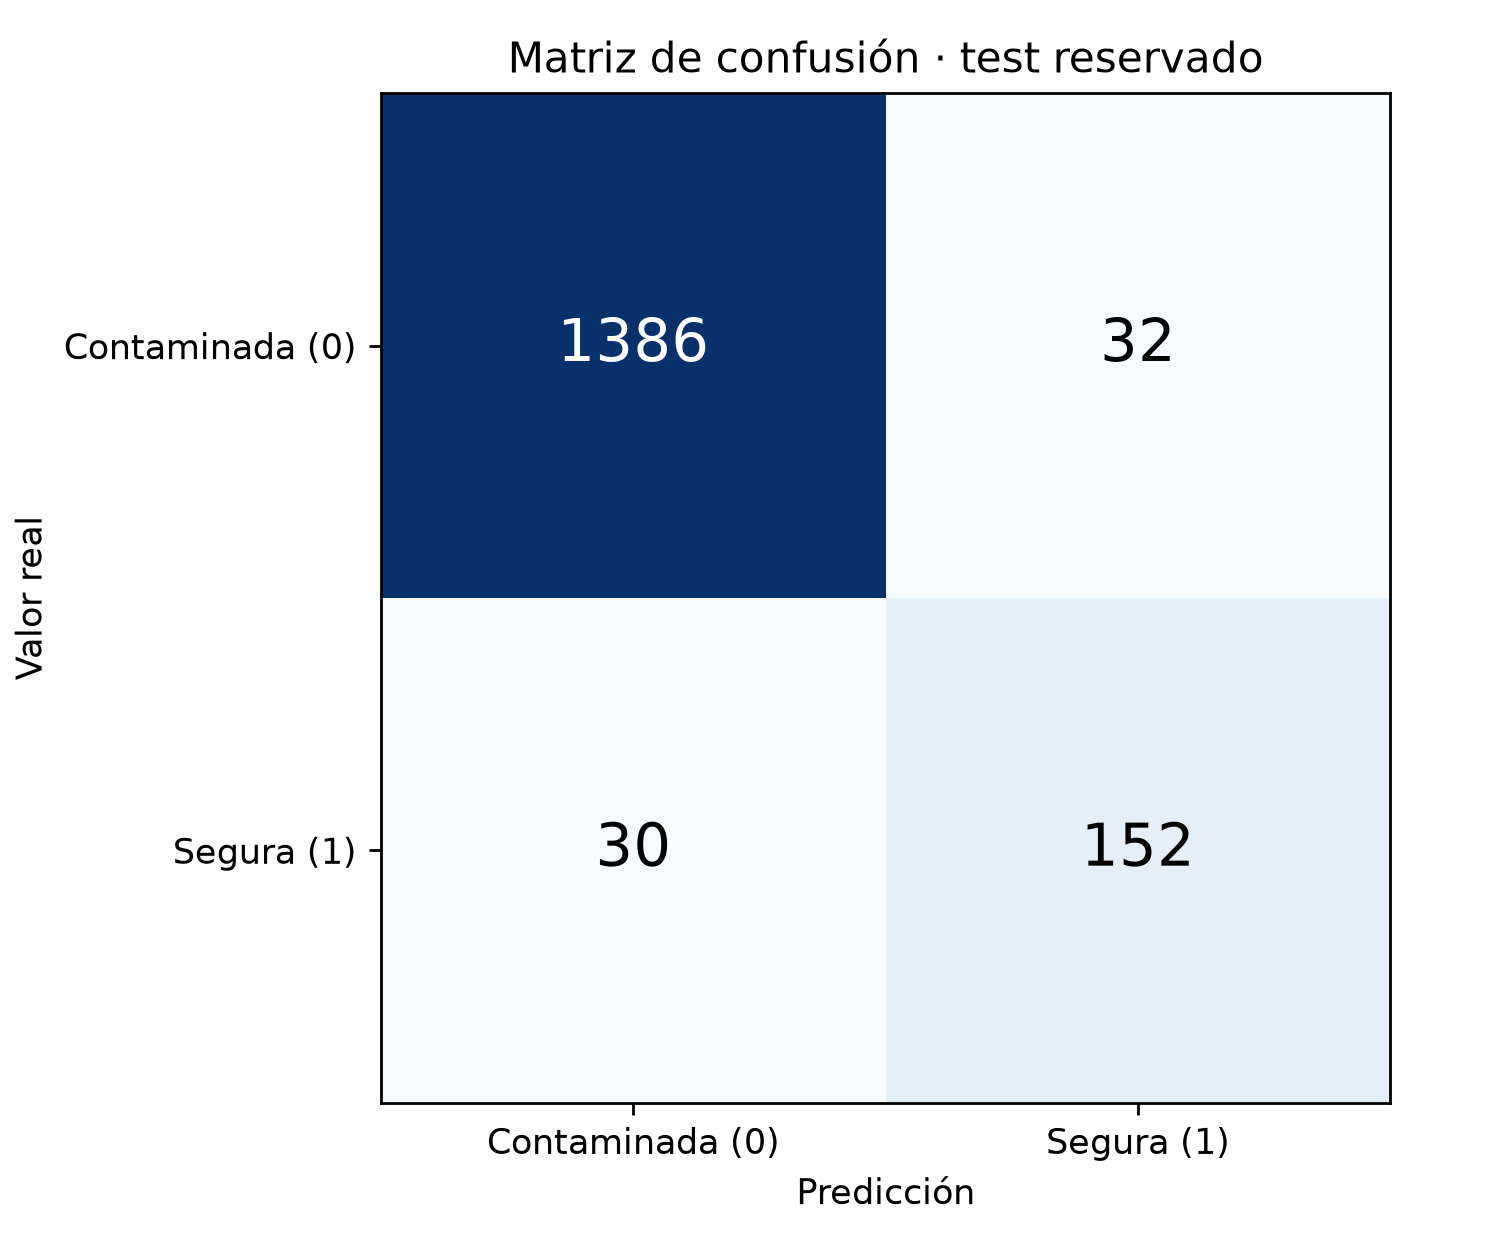
\includegraphics[width=.62\textwidth,height=5.4cm,keepaspectratio]{reports/figures/08_test_confusion_matrix.png}\\[0.12cm]
{\small\textbf{Figura 7.} Matriz de confusi\'{o}n del modelo final Random Forest optimizado con GA evaluado sobre el conjunto de prueba independiente (1.600 muestras).}
\end{center}

\clearpage
\section*{8. Prototipo y demostración}
FastAPI (backend/api.py) carga models/final\_pipeline.joblib y los metadatos guardados. React/Vite (frontend/) permite editar las veinte variables y consultar la API. La interfaz obtiene los perfiles desde el backend y los datos se reordenan según feature\_order. El build se sirve desde FastAPI en el puerto 8000. El README describe instalación y pruebas.

{\small\begin{tabularx}{\textwidth}{XX}
\toprule
Caso & Resultado esperado y alcance \\
\midrule
A: perfil de train & Clase 1 sin excesos en las comparaciones implementadas. No certifica potabilidad. \\
B: metales y nitrato alto & Clase 0, alertas y nitrato fuera del rango train (55 > 19,83). \\
C: extremo adverso & Clase 1 con alertas y extrapolación. Falla conocida, marcada como conflicto. \\
Entradas inválidas & Vacíos, texto, negativos, NaN, infinitos y booleanos se rechazan antes de inferir. \\
\bottomrule\end{tabularx}}

Las probabilidades se muestran como scores de clase no calibrados. Las comparaciones con valores guía OMS [8] son condicionales a confirmar mg/L, especie química y método. No se asignan unidades radiológicas ni microbiológicas sin evidencia. El mercurio no se compara por falta de especiación. Las alertas no modifican la etiqueta del modelo.

\vspace{0.2cm}
\begin{center}
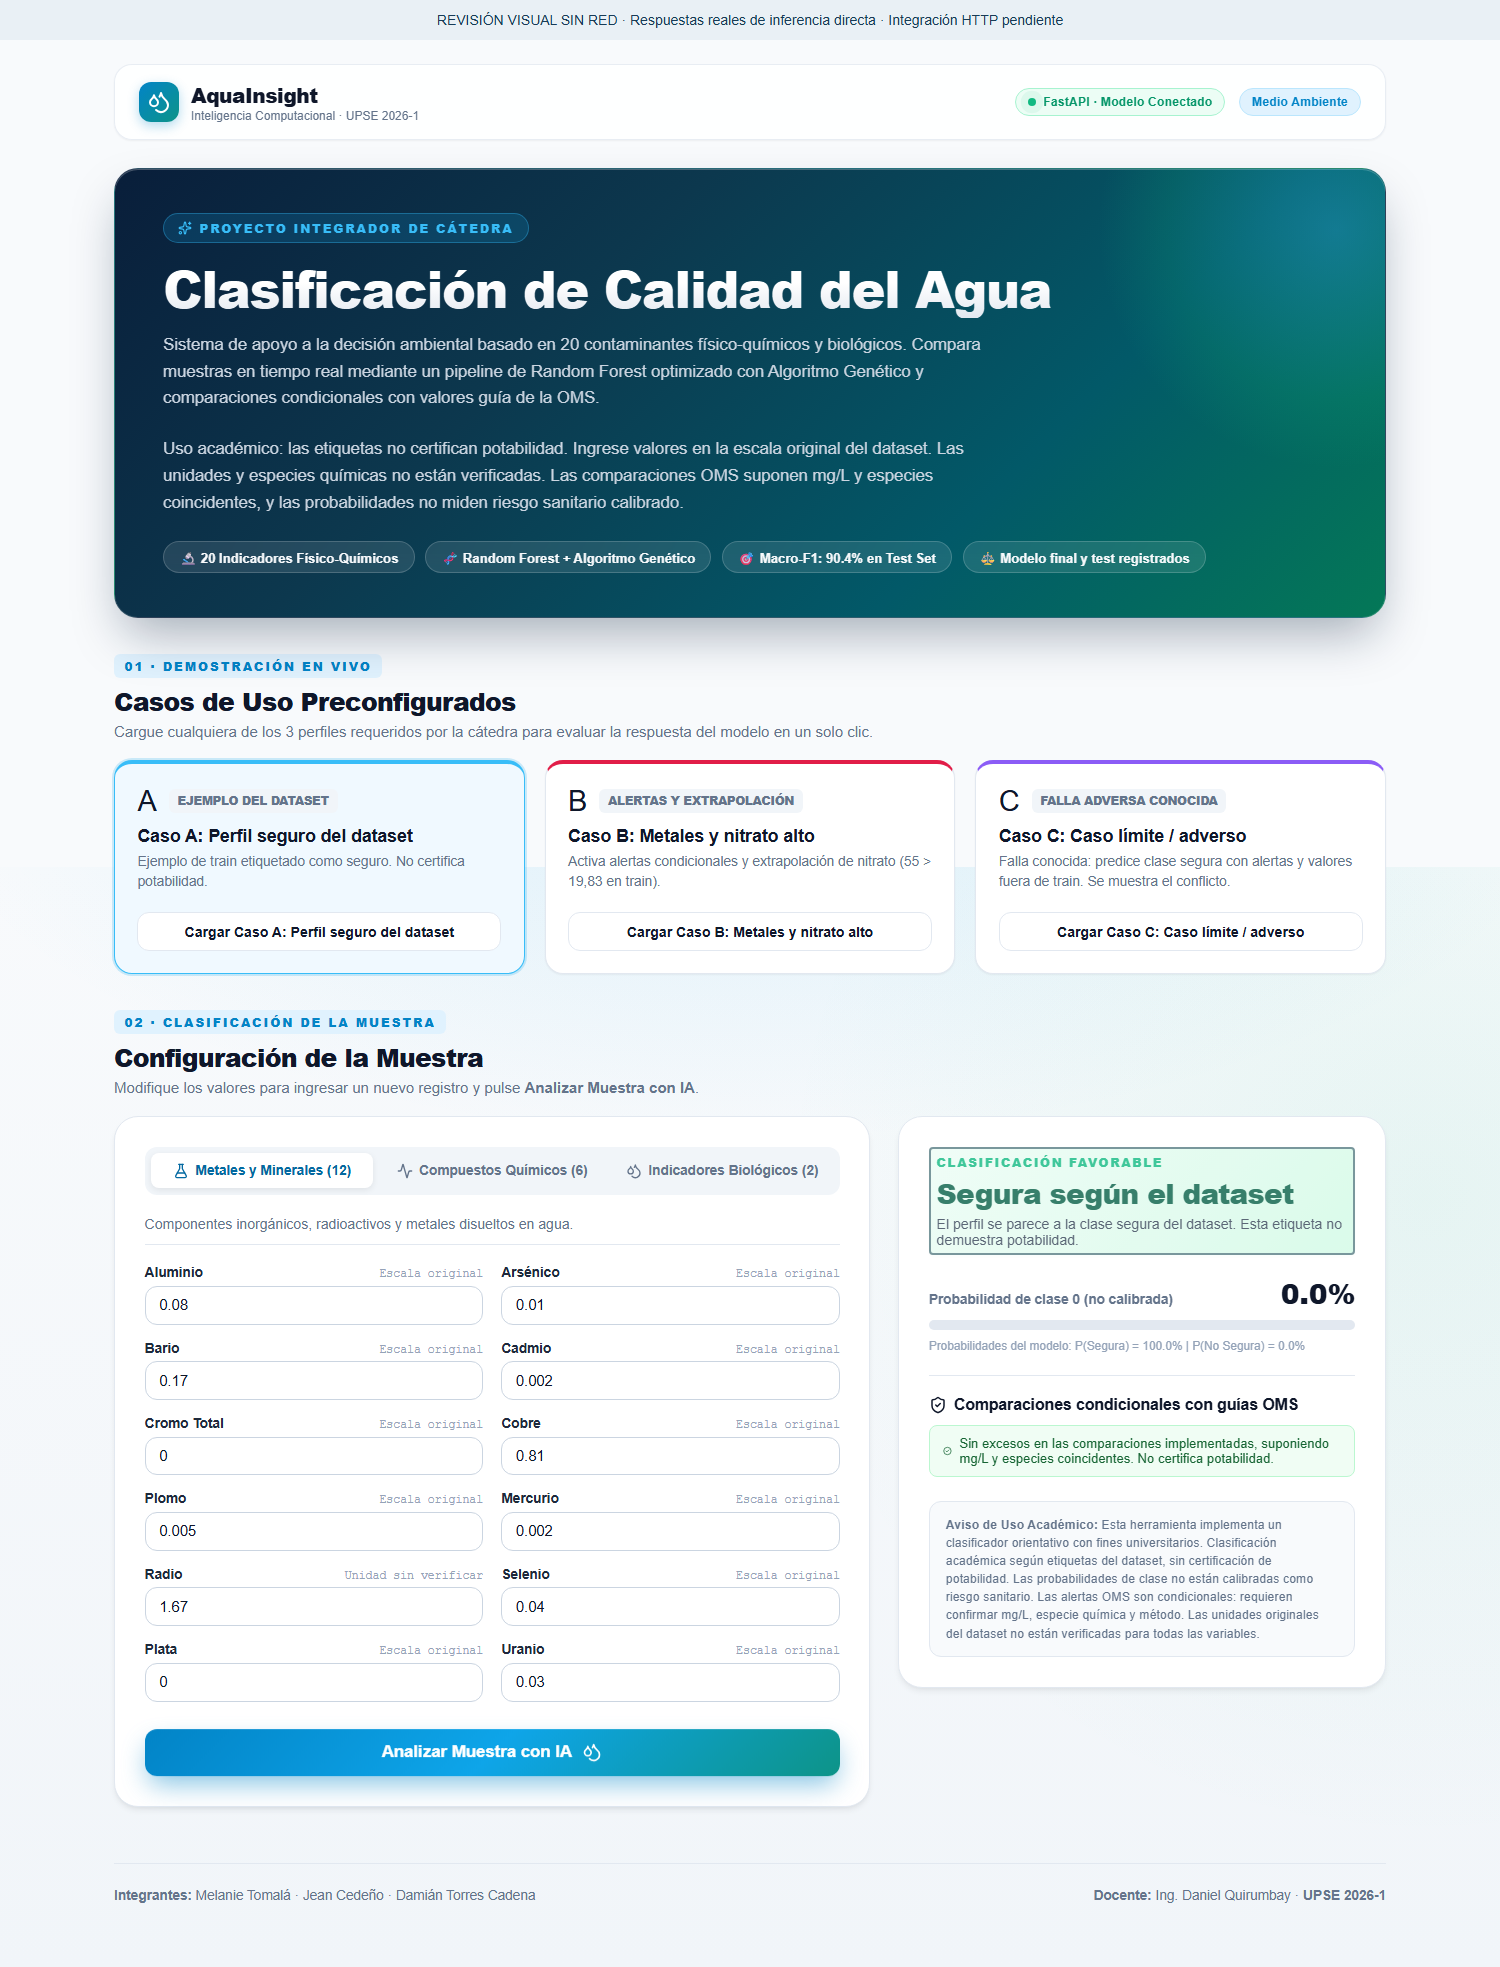
\includegraphics[width=.48\textwidth,height=6.8cm,keepaspectratio]{reports/evidence/case_a_safe.png}
\hfill
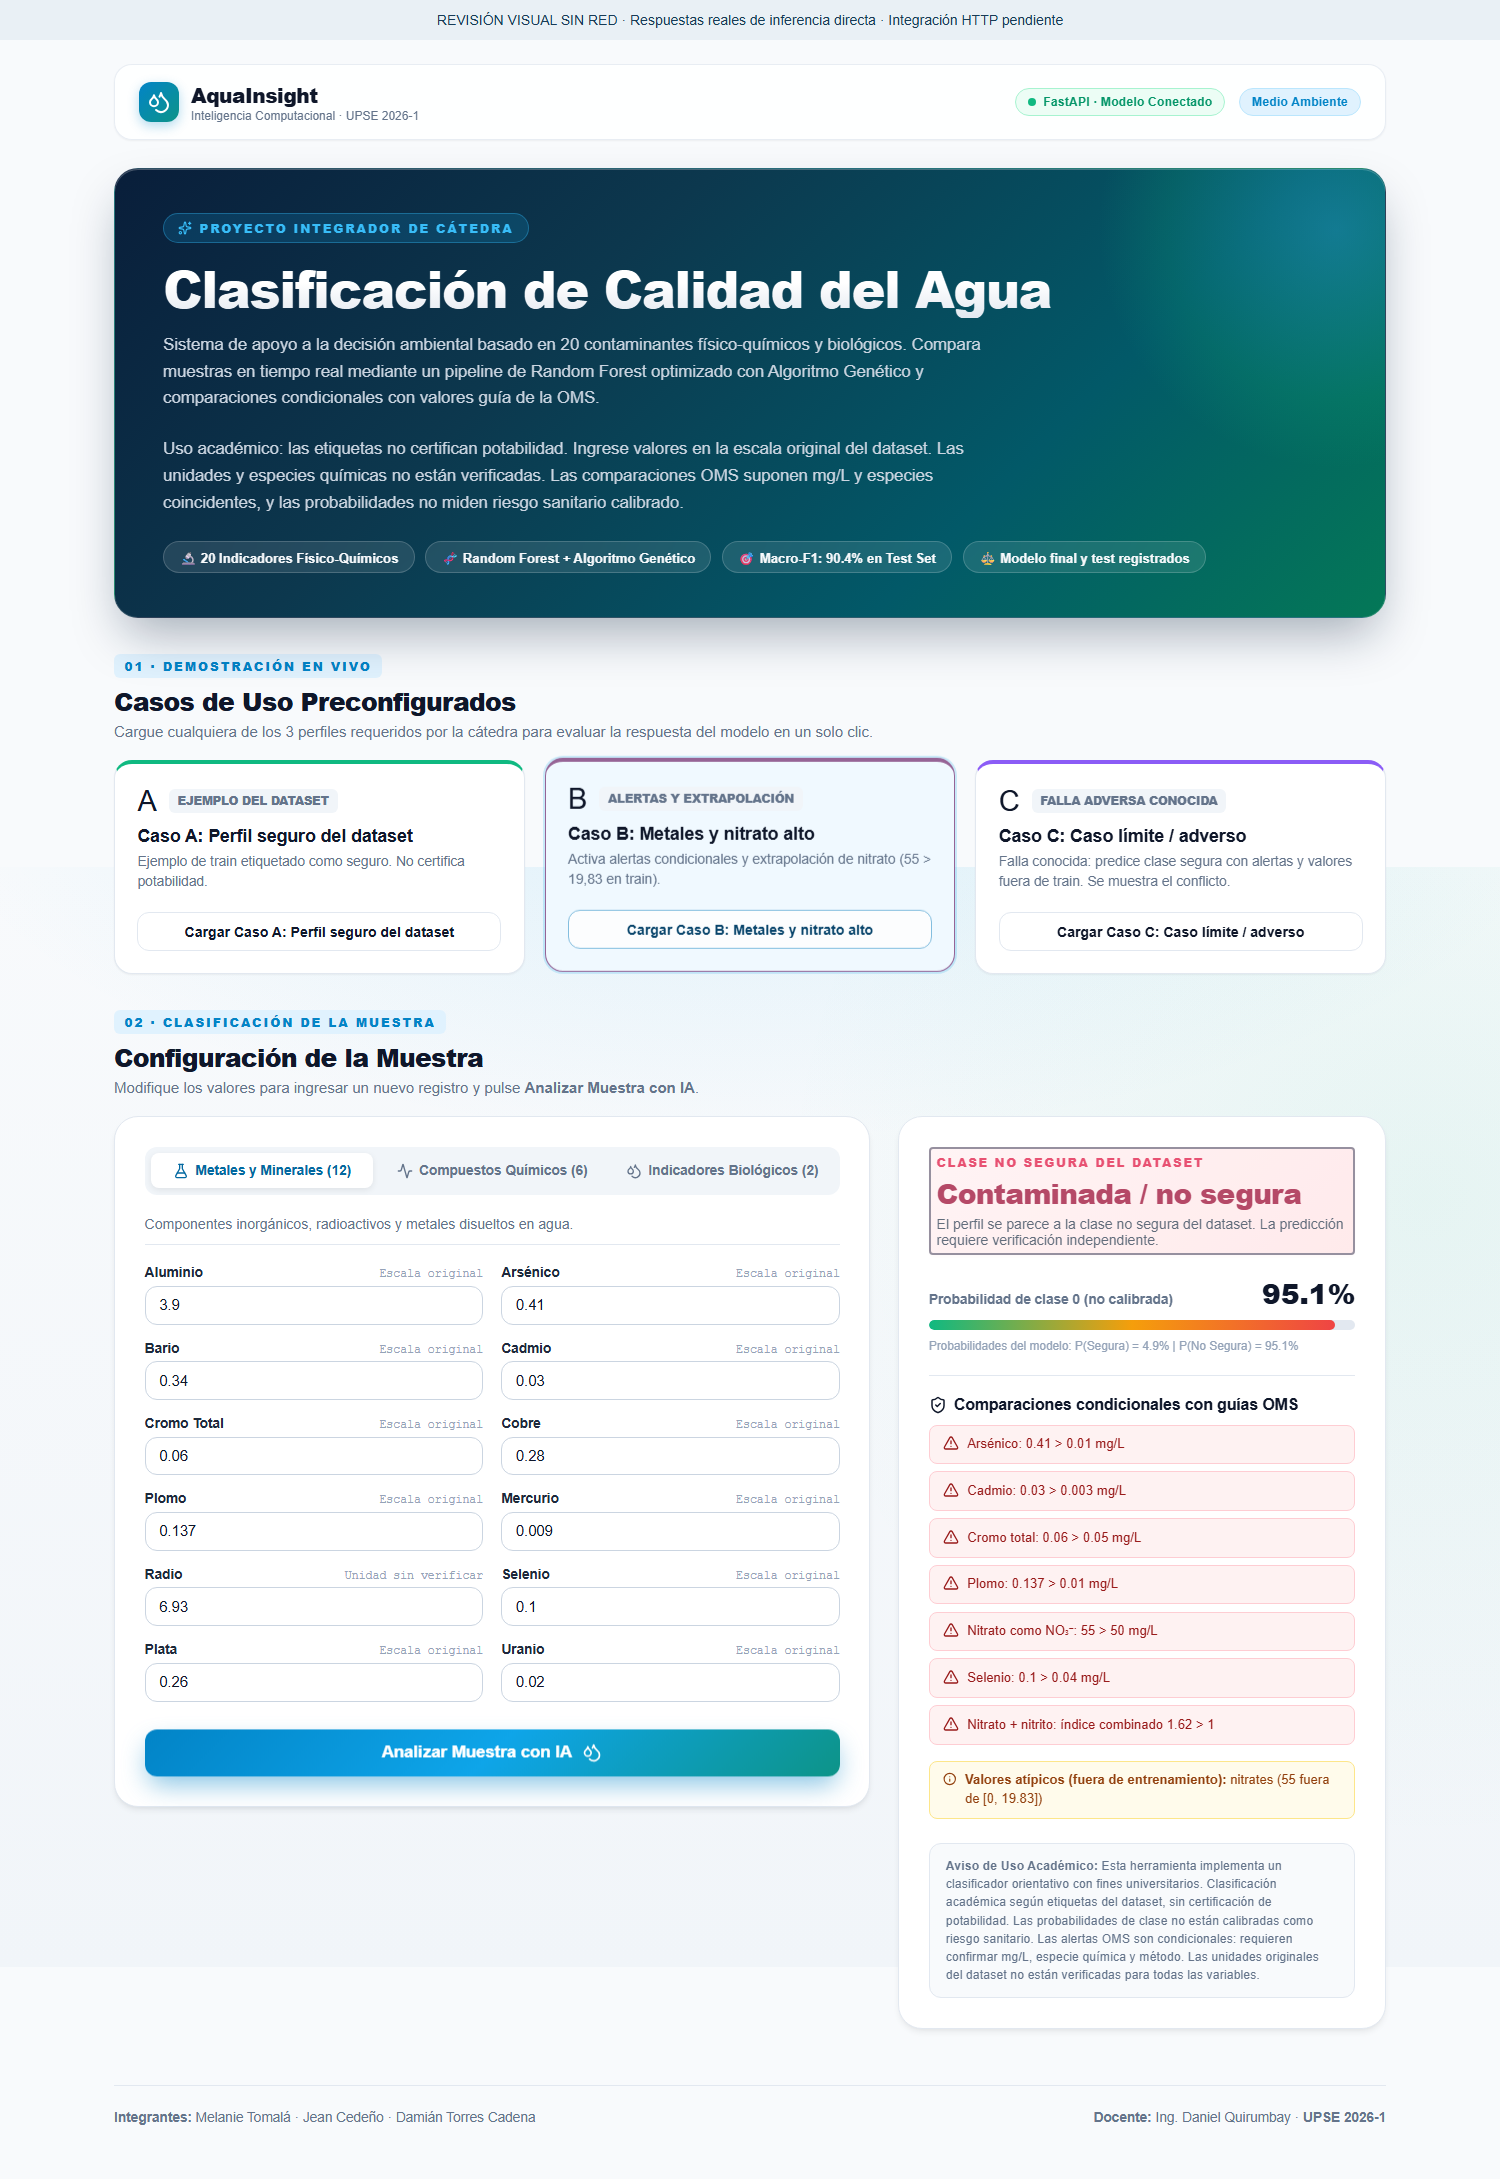
\includegraphics[width=.48\textwidth,height=6.8cm,keepaspectratio]{reports/evidence/case_b_contaminated.png}\\[0.12cm]
{\small\textbf{Figura 8.} Interfaz del prototipo web (AquaInsight): Caso A (izquierda, perfil de entrenamiento seguro) y Caso B (derecha, muestra contaminada con alertas normativas).}
\end{center}

Verificación de esta revisión: las pruebas directas de esquema e inferencia usan el pipeline real. La revisión visual del navegador utiliza respuestas grabadas de esas inferencias, sin red. El host rechaza conexiones a 127.0.0.1 (EACCES), por lo que la integración HTTP no pudo verificarse aquí. Las capturas son evidencia de interfaz con esas respuestas, no una prueba del transporte HTTP. Se debe completar esa comprobación en el equipo de defensa.

Durante la defensa debe modificarse al menos un valor de un perfil y ejecutar Analizar Muestra con IA. Los tres ejemplos preconfigurados muestran comportamiento, pero no sustituyen ese registro nuevo. El caso C evidencia una limitación de extrapolación y no se elimina ni se fuerza a clase 0 para mejorar la demostración.

\vspace{0.2cm}
\begin{center}
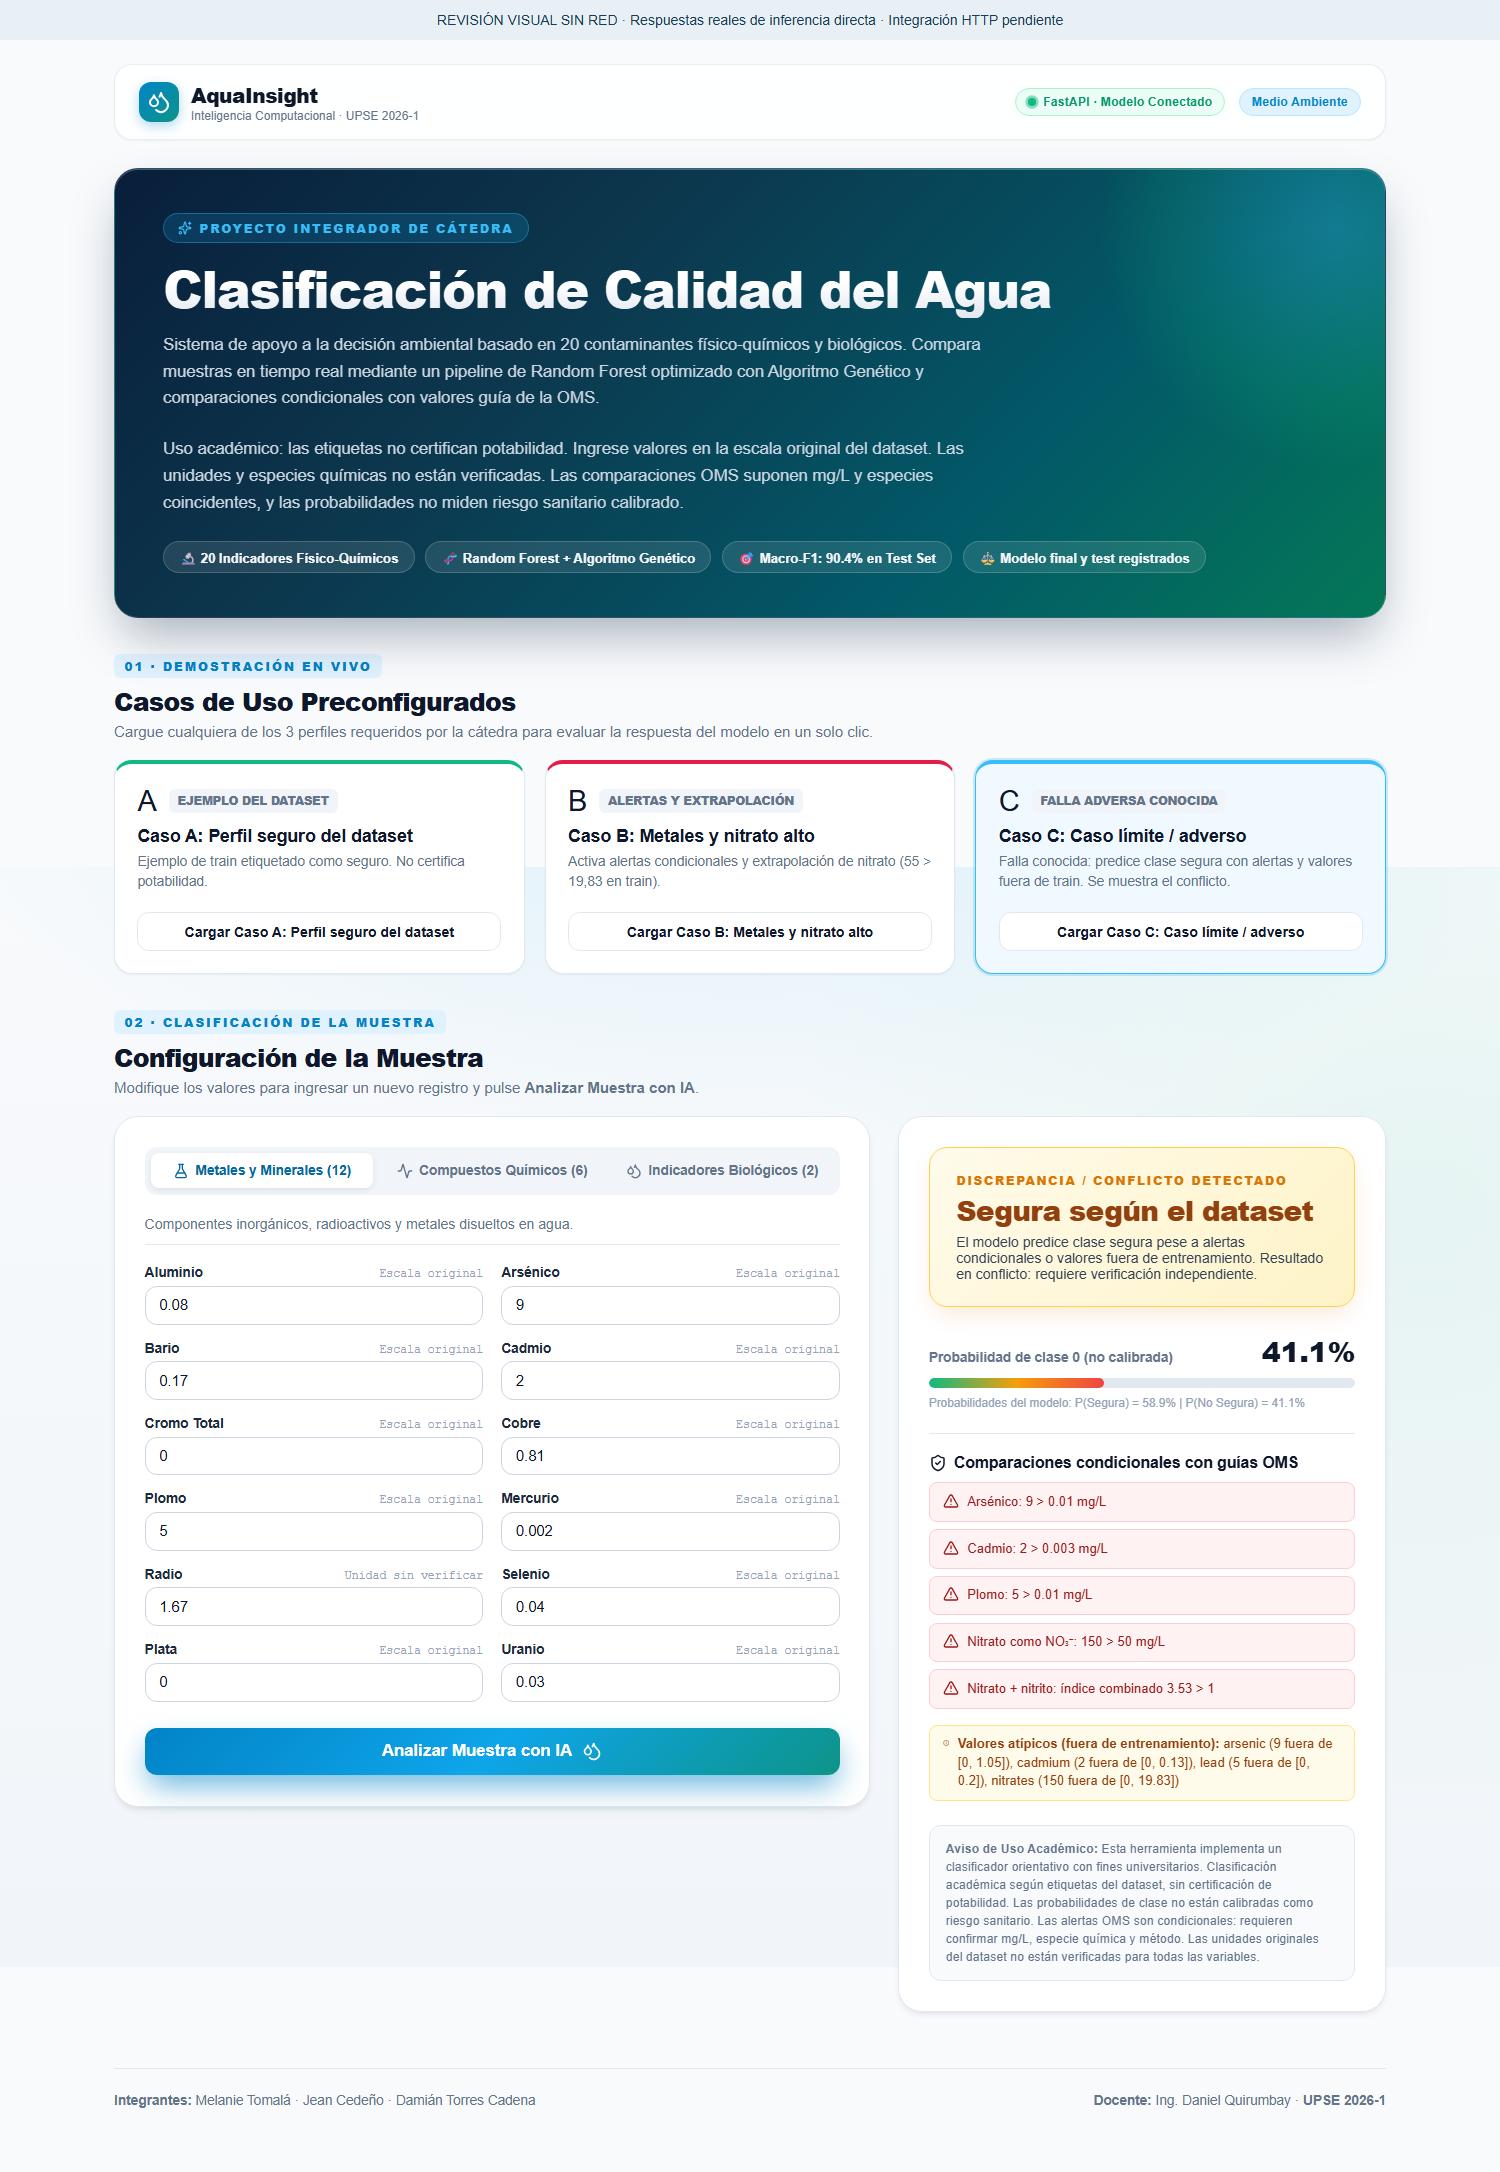
\includegraphics[width=.52\textwidth,height=6.8cm,keepaspectratio]{reports/evidence/case_c_adversarial.png}\\[0.2cm]
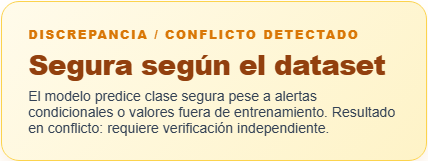
\includegraphics[width=.6\textwidth,height=2cm,keepaspectratio]{reports/evidence/case_c_banner.png}\\[0.12cm]
{\small\textbf{Figura 9.} Caso C (extremo adverso): evidencia de extrapolaci\'{o}n cr\'{i}tica y banner de conflicto entre el score del clasificador y l\'{i}mites de gu\'{i}a sanitaria.}
\end{center}

\clearpage
\section*{9. Discusión, conclusiones y mejoras}
El criterio de superar a Dummy en Macro-F1 de CV se cumple para los cuatro modelos evaluados. Los bosques presentan las mayores medias en esta ejecución. La búsqueda convencional alcanza una media ligeramente mayor que el GA y utiliza menos tiempo total registrado. Estos resultados no respaldan una ventaja universal de la metaheurística.

El proyecto evidencia los tres ejes de inteligencia computacional: compara una MLP, aplica un GA e investiga lógica difusa, junto con un manejo práctico de incertidumbre mediante rangos, scores y conflictos. Se declara expresamente que no se implementó inferencia Mamdani ni calibración de riesgo sanitario.

Sesgos y limitaciones: desbalance 89/11, origen y mecanismos de etiquetado poco documentados, ausencia de identificadores temporales y de entidad, incertidumbre sobre unidades y mediciones negativas. El análisis exploratorio previo al split y la inspección de una fila de test impiden afirmar un sellado absoluto, aunque no se usó el test para ajustar transformaciones ni seleccionar el candidato final.

La reutilización de CV durante búsqueda puede sobreestimar candidatos optimizados. Se ejecutó una sola semilla y los presupuestos no fueron equivalentes. El resultado adverso demuestra que un valor extremo puede producir una etiqueta aparentemente favorable. Por ello el sistema no debe usarse para decidir consumo humano ni reemplazar ensayos acreditados.

Mejoras futuras: adquirir datos independientes con unidades, ubicación, fecha y protocolo de laboratorio verificables; diseñar particiones por tiempo o entidad; comparar búsquedas con presupuestos iguales y varias semillas; evaluar calibración, rechazo por dominio y, si procede, reglas difusas validadas por especialistas. Estas mejoras requieren un nuevo protocolo experimental y nueva prueba externa, conservando el test actual como resultado ya conocido.

Conclusión: se construyó un flujo reproducible de clasificación, comparación, optimización e inferencia para fines académicos. El pipeline seleccionado se conserva y el prototipo muestra sus predicciones con sus limitaciones. El cierre científico depende de comprender errores y alcance, además de presentar métricas agregadas.

Declaración de IA generativa: se empleó OpenAI Codex para apoyar programación, revisión documental, pruebas y preparación de entregables. El borrador previo también declara asistencia de Google Antigravity. El equipo debe revisar y confirmar esa declaración y el anexo de contribuciones antes de presentar; no se atribuyen tareas individuales ni validaciones humanas que no hayan sido confirmadas.

\clearpage
\section*{Referencias}
[1] T. M. Cover y P. E. Hart, ``Nearest neighbor pattern classification,'' \textit{IEEE Transactions on Information Theory}, vol. 13, no. 1, pp. 21-27, 1967.\newline \url{https://doi.org/10.1109/TIT.1967.1053964}

[2] C. Cortes y V. Vapnik, ``Support-vector networks,'' \textit{Machine Learning}, vol. 20, pp. 273-297, 1995.\newline \url{https://doi.org/10.1007/BF00994018}

[3] L. Breiman, ``Random Forests,'' \textit{Machine Learning}, vol. 45, pp. 5-32, 2001.\newline \url{https://doi.org/10.1023/A:1010933404324}

[4] D. E. Rumelhart, G. E. Hinton y R. J. Williams, ``Learning representations by back-propagating errors,'' \textit{Nature}, vol. 323, pp. 533-536, 1986.\newline \url{https://doi.org/10.1038/323533a0}

[5] J. H. Holland, \textit{Adaptation in Natural and Artificial Systems}. Cambridge, MA: MIT Press, 1992.\newline \url{https://doi.org/10.7551/mitpress/1090.001.0001}

[6] L. A. Zadeh, ``Fuzzy sets,'' \textit{Information and Control}, vol. 8, no. 3, pp. 338-353, 1965.\newline \url{https://doi.org/10.1016/S0019-9958(65)90241-X}

[7] L. Grb\v{c}i\'{c} et al., ``Coastal water quality prediction based on machine learning with feature interpretation and spatio-temporal analysis,'' arXiv:2107.03230v2, 2021. Prepublicación.\newline \url{https://doi.org/10.48550/arXiv.2107.03230}

[8] Organización Mundial de la Salud, \textit{Guidelines for drinking-water quality: fourth edition incorporating the first, second and third addenda}. Ginebra: OMS, 2026.\newline \url{https://www.who.int/publications/i/item/9789240121225}

Fuentes primarias verificadas el 21/10/2026: publicaciones editoriales para [1]-[6], prepublicación identificada para [7] y documento oficial OMS para [8]. Las referencias sustentan el método y el contexto, sin transferir sus resultados a este dataset. Los metadatos de algunas referencias del borrador anterior no coincidían con los DOI y se sustituyeron.

Datos: mssmartypants, Water Quality, Kaggle. \url{https://www.kaggle.com/datasets/mssmartypants/water-quality}. Consulta inicial 20/10/2026. Resultados propios: reports/phase3\_results.json y reports/phase4\_selection.json.

\end{document}
